\part{Dynamics}
    \section{Dynamics}
    \subsection{Dynamics in Classical Mechanics}
    In classical mechanics the dynamics of a system can be entirely determined from Newton's second law:
    \[\vv{F} = m\vv{a} = m\dv[2]{\vv{r}}{t}.\]
    The force term encodes information about the external forces applied to the system, the mass is a characteristic of the system and the acceleration provides a time dependence.
    Solving this differential equation can give us the equations of motion.
    From these we can predict the future of the system but also the past.
    
    \subsection{Dynamics in Quantum Mechanics}
    \begin{postulate}{}{}
        The dynamics of a system described by the state \(\ket{\Psi(t)}\), at time \(t\), is determined by the \define{Schr\"odinger equation}:
        \[i\hbar\dv{t}\ket{\Psi(t)} = \operator{H}\ket{\Psi(t)}.\]
        Where \(\operator{H}\) is the \define{Hamiltonian}, a hermitian operator corresponding to the energy of the system.
    \end{postulate}
    The state vectors, \(\ket{\Psi(t)}\), now include an explicit time dependence.
    
    The Hamiltonian, for a single particle in one dimension, is given in an analogous way to classical mechanics by
    \[\operator{H} = \operator{T} + \operator{V}.\]
    Here \(\operator{T}\) is the operator associated with the kinetic energy and \(\operator{V}\) is the operator associated with the potential energy.
    In general it is often possible to take a classical formula and change \(x\) to \(\operator{X}\), and \(p\) to \(\operator{P}\) and have it still be valid, although we do have to be careful about whether operators commute which we don't have to consider with classical mechanics.
    Fortunately this is valid for this case and we have
    \begin{align*}
        T = \frac{p^2}{2m} &\rightarrow \operator{T} = \frac{\operator{P}^2}{2m},\\
        V = V(x) &\rightarrow \operator{V} = V(\operator{X}).
    \end{align*}
    Here the function \(V\) on the left, which acts on real numbers, and the function \(V\) on the right, which acts on operators, are technically different as their domains are different but they have the same form.
    For example in a harmonic potential,
    \[V(x) = \frac{1}{2}kx^2\]
    and the operator equivalent is
    \[V(\operator{X}) = \frac{1}{2}k\operator{X}^2.\]
    Consider a state \(\ket{\Psi(t)}\), after a small amount of time, \(\varepsilon\), this becomes
    \begin{align*}
        \ket{\Psi(t + \varepsilon)} &= \ket{\Psi(t)} + \varepsilon\dv{t}\ket{\Psi(t)}\\
        &= \ket{\Psi(t)} - \frac{i\varepsilon}{\hbar}\operator{H}\ket{\Psi(t)}
    \end{align*}
    In this way we can view the change in time as the result of the action of \(\operator{H}\).
    
    \subsection{Time Evolution of a Wave Function}
    The wave function related to the state \(\ket{\Psi(t)}\) is, as normal, found by the inner product with the position eigenbasis vectors:
    \[\Psi(x, t) = \braket{x}{\Psi(t)}.\]
    If we take the inner product of the left hand side of the Schr\"odinger equation with one of these basis vectors we get
    \[\bra{x}i\hbar\dv{t}\ket{\Psi(t)} = i\hbar\dv{t}\braket{x}{\Psi(t)} = i\hbar\pdv{t}\Psi(x, t).\]
    Here we have used the fact that \(\bra{x}\) is independent of time so commutes with a time derivative.
    Taking the inner product with the right hand side we have
    \[\bra{x}\operator{H}\ket{\Psi(t)} = \operator{H}\braket{x}{\Psi(t)} = \operator{H}\Psi(x, t).\]
    
    In the case that \(\operator{H} = \operator{T} + \operator{V}\),
    \[\operator{T} = \frac{\operator{P}^2}{2m},\qquad\text{and}\qquad \operator{V} = V(\operator{X})\]
    the Schr\"odinger equation becomes
    \[\operator{H}\Psi(x, t) = \left[\frac{\operator{P^2}}{2m} + V(\operator{X})\right]\Psi(x, t) = i\hbar\pdv{t}\Psi(x, t).\]
    We can calculate the action of \(\operator{P}^2\Psi(x, t)\) easily:
    \[\operator{P}^2\Psi(x, t) = -i\hbar\pdv{x}\left(-i\pdv{x}\hbar\right) = -\hbar^2\pdv[2]{x}\Psi(x, t).\]
    Since the action of \(\operator{X}\) is simply multiplication by \(x\) we have that \(V(\operator{X}) = V(x)\).
    Schr\"odinger's equation becomes
    \[\left[-\frac{\hbar^2}{2m}\pdv[2]{x} + V(x)\right]\Psi(x, t) = i\hbar\pdv{t}\Psi(x, t).\]
    Notice that this has a second order derivative with respect to position but only a first order derivative with respect to time.
    This means that time and position are treated differently and therefore this formula fails to be relativistic.
    
    \subsection{Justification of the Schr\"odinger Equation}
    While the Schr\"odinger equation is a postulate so doesn't need justifying it can't hurt to take a brief look at the logic that one could apply in coming up with it in the first case.
    A plane wave has the wave function
    \[\Psi(x, t) = Ae^{-i(\omega t - kx).}\]
    This describes the propagation of monochromatic light.
    Applying \(i\hbar\partial_t\) to this we get
    \begin{align*}
        i\hbar\pdv{t}\Psi(x, t) &= i\hbar\pdv{t}Ae^{-i(\omega t - kx).}\\
        &= i\hbar(-i\omega t)Ae^{-i(\omega t - kx).}\\
        &= \hbar\omega\Psi(x, t)\\
        &= 2\pi\nu\hbar\Psi(x, t)
    \end{align*}
    where \(\nu = \omega/2\pi\) is the frequency of the wave.
    The eigenvalue, \(2\pi\nu\hbar\), is precisely the energy of the photon which justifies the use of the Hamiltonian as the operator associated with the total energy.
    
    As well as this we also require \(\norm{\Psi(t)} = 1\) for all times, \(t\):
    \[\norm{\Psi(t)}^2 = \int\dd{x} \Psi^*(x, t)\Psi(x, t) = 1.\]
    Since this integral is constant with respect to time the time derivative of this integral must vanish:
    \begin{align*}
        0 &= \dv{t}\int\dd{x}\Psi^*(x, t)\Psi(x, t)\\
        &= \int\dd{x}\pdv{t}[\Psi^*(x, t)\Psi(x, t)]\\
        &= \int\dd{x}\left[\left(\pdv{t}\Psi^*(x, t)\right)\Psi(x, t) + \Psi^*(x, t)\left(\pdv{t}\Psi(x, t)\right)\right]
    \end{align*}
    This occurs if \(\partial_t\) is represented by an anti-hermitian operator.
    This is why there is a factor of \(i\), since if \(A\) is anti-hermitian then \(iA\) is hermitian so \(i\partial_t\) is represented by a hermitian operator.
    The factor of \(\hbar\) is required for the dimensions to match correctly.
    
    \subsection{Eigenstates of the Hamiltonian}
    The Hamiltonian is the operator associated with the energy.
    Assuming that the spectrum of \(\operator{H}\) is discrete the eigenvalue equation for \(\operator{H}\) is
    \begin{empheq}[box=\tcbhighmath]{equation*}
        \operator{H}\ket{\psi_n} = E_n\ket{\psi_n}.
    \end{empheq}
    This is called the \define{\gls{tise}}.
    \(E_n\in\reals\) are the possible outcomes of measuring the energy of the system and \(\ket{\psi_n}\) is a state in which, when measuring the energy, we get \(E_n\) with probability 1.
    
    \subsubsection{Time Evolution of the Energy Eigenstates}
    Suppose we have a system that starts in one of the energy eigenstates.
    That is
    \[\ket{\Psi(0)} = \ket{\psi_n}.\]
    We make the ansatz that the time evolution of the system, that is the state of the system after some time, \(t\), is given by
    \[\ket{\Psi(t)} = e^{-iE_nt/\hbar}\ket{\Psi(0)} = e^{-iE_nt/\hbar}\ket{\psi_n}.\]
    We can easily check that this satisfies the Schr\"odinger equation:
    \begin{align*}
        i\hbar\dv{t}\ket{\Psi(t)} &= i\hbar\dv{t}\left(e^{-iE_nt/\hbar}\ket{\psi_n}\right)\\
        &= i\hbar\ket{\psi_n}\left(\dv{t}e^{-iE_nt/\hbar}\right)\\
        &= i\hbar\ket{\psi_n} \left( -\frac{i}{\hbar}E_ne^{-iE_nt/\hbar} \right)\\
        &= E_ne^{-iE_nt/\hbar}\ket{\psi_n}\\
        &= e^{-iE_nt/\hbar}\operator{H}\ket{\psi_n}\\
        &= \operator{H}\ket{\Psi(t)}.
    \end{align*}
    Here we have used the fact that the state, \(\ket{\psi_n}\), is independent of time so commutes with \(\inlinedv{}{t}\).
    Also the phase factor, \(\exp(-iE_nt/\hbar)\in\complex\), commutes with the operator \(\operator{H}\).
    
    This also trivially satisfies the boundary conditions:
    \[\ket{\Psi(0)} = e^{-iE_n0/\hbar}\ket{\psi_n} = \ket{\psi_n}.\]
    Hence we conclude that the ansatz is correct.
    
    \subsubsection{Time Evolution of Matrix Elements}
    Let \(\operator{O}\) be a generic operator that is constant with respect to time.
    Define the matrix element
    \[O_n(t) = \bra{\Psi_n(t)}\operator{O}\ket{\Psi_n(t)}\]
    where
    \[\ket{\Psi_n(t)} = e^{-iE_nt/\hbar}\ket{\psi_n}.\]
    This gives us
    \[\bra{\Psi_n(t)} = e^{iE_nt/\hbar}\bra{\psi_n}.\]
    Notice that \(O_n(t)\) may have time dependence as the states have time dependence even if the operator doesn't.
    However it actually turns out that \(O_n(t)\) \emph{doesn't} have time dependence:
    \begin{align*}
        O_n(t) &= \bra{\Psi_n(t)}\operator{O}\ket{\Psi_n(t)}\\
        &= \bra{\psi_n} e^{iE_nt/\hbar} \operator{O} e^{-iE_nt/\hbar} \ket{\psi_n}\\
        &= \bra{\psi_n}\operator{O}\ket{\psi_n}\\
        &= O_n(0).
    \end{align*}
    Hence \(O_n(t)\) is independent of \(t\).
    Here we have used that the phase factors are simply complex numbers so commute with the operators.
    
    We can conclude that when the system is prepared in an eigenstate of the Hamiltonian all expected values of operators are constant.
    For this reason we call \(\ket{\psi_n}\) \define{stationary states}.
    
    \begin{example}
        Consider the operator \(\operator{\proj}_x = \ketbra{x}{x}\).
        The matrix element of this is
        \[\bra{\Psi(t)}\operator{\proj}_x\ket{\Psi(t)} = \braket{\Psi(t)}{x}\braket{x}{\Psi(t)} = \abs{\Psi(x, t)}^2.\]
        This must be independent of time if \(\ket{\Psi(0)} = \ket{\psi_n}.\)
        As usual \(\abs{\Psi(x, t)}^2\) gives the probability of finding the system at \(x\).
        Since this is independent of time the expected position of \(x\) is constant.
        This justifies the name `stationary state'.
    \end{example}
    
    \subsection{Time Evolution of a Generic State}
    We define a \define{time evolution operator}, \(\operator{U}(t)\), that acts on a state at time \(t = 0\) to give the value of that state at time \(t\):
    \[\operator{U}(t)\ket{\Psi(0)} = \ket{\Psi(t)}.\]
    The form of this operator is
    \[\operator{U}(t) = \exp\left(-\frac{i}{\hbar}\operator{H}t\right).\]
    Notice the similarity to the time evolution of a single state.
    All that has happened is the eigenvalue has been replaced by the operator.
    As usual with operators the exponential is defined through its Taylor series:
    \[\exp\left(-\frac{i}{\hbar}\operator{H}t\right) = \sum_{k=0}^{\infty} \frac{1}{k!}\left(-\frac{i}{\hbar}\right)^k \operator{H}^k t^k\]
    We can show that
    \[\operator{U}(t)\ket{\Psi(0)}\]
    is a solution to the Schr\"odinger equation:
    \begin{align*}
        i\hbar\dv{t}\operator{U}\ket{\Psi(0)} &= i\hbar\dv{t} \exp\left(-\frac{i}{\hbar}\operator{H}t\right) \ket{\Psi(0)}\\
        &= i\hbar \dv{t} \sum_{k=0}^{\infty} \frac{1}{k!}\left(-\frac{i}{\hbar}\right)^k \operator{H}^k t^k \ket{\Psi(0)}
        \shortintertext{Note that only the terms \(t^k\) have time dependnece:}
        &= i\hbar \sum_{k=0}^{\infty} \frac{1}{k!}\left(-\frac{i}{\hbar}\right)^k \operator{H}^k \ket{\Psi(0)} \dv{t} t^k\\
        &= i\hbar \sum_{k=0}^{\infty} \frac{1}{k!}\left(-\frac{i}{\hbar}\right)^k \operator{H}^k \ket{\Psi(0)} k t^{k-1}
        \shortintertext{The first term in the sum is zero so we can disregard it}
        &= i\hbar \sum_{k=1}^{\infty} \frac{1}{k!}\left(-\frac{i}{\hbar}\right)^k \operator{H}^k \ket{\Psi(0)} k t^{k-1}\\
        &= i\hbar \sum_{k=1}^{\infty} \frac{1}{(k-1)!}\left(-\frac{i}{\hbar}\right)^k \operator{H}^k \ket{\Psi(0)} t^{k-1}\\
        &= \sum_{k=1}^{\infty} \frac{1}{(k-1)!}\left(-\frac{i}{\hbar}\right)^{k-1} \operator{H}^k \ket{\Psi(0)}  t^{k-1}\\
        &= \operator{H} \sum_{k=1}^{\infty} \frac{1}{(k-1)!}\left(-\frac{i}{\hbar}\right)^{k-1} \operator{H}^{k-1} \ket{\Psi(0)}  t^{k-1}
        \shortintertext{Let \(k' = k - 1\):}
        &= \operator{H} \sum_{k'=0}^{\infty} \frac{1}{k'!}\left(-\frac{i}{\hbar}\right)^{k'} \operator{H}^{k'} \ket{\Psi(0)} t^{k'}\\
        &= \operator{H} \exp\left(-\frac{i}{\hbar}\operator{H}t\right) \ket{\Psi(0)}.\\
        &= \operator{H}\operator{U}(t)\ket{\Psi(0)}.
    \end{align*}
    Hence \(\operator{U}(t)\ket{\Psi(0)}\) is a solution to the Schr\"odinger equation with the boundary condition that \(U(0)\ket{\Psi(0)} = \ket{\Psi(0)}\).
    Note that in showing this we assumed nothing about the derivative of \(e^{\operator{A}t}\).
    We have shown that derivative is the same as if \(\operator{A}\) was a constant real number, that is
    \[\dv{t}e^{\operator{A}t} = \operator{A}e^{\operator{A}t}.\]
    From now on we will assume this.
    
    We can use this to recover the time evolution of the eigenbasis of the Hamiltonian:
    \begin{align*}
        \operator{U}(t)\ket{\psi_n} &= \exp\left(-\frac{i}{\hbar}\operator{H}t\right) \ket{\psi_n}\\
        &= \sum_{k=0}^{\infty} \frac{1}{k!}\left(-\frac{i}{\hbar}\right)^k t^k\operator{H}^k \ket{\psi_n}\\
        &= \sum_{k=0}^{\infty} \frac{1}{k!}\left(-\frac{i}{\hbar}\right)^k t^kE_n^k \ket{\psi_n}\\
        &= \exp\left(-\frac{i}{\hbar}E_nt\right) \ket{\psi_n}\\
    \end{align*}
    
    \subsection{The Eigenbasis of the Hamiltonian}
    For any mildly complex system the form of the Hamiltonian can make actually calculating the time evolution operator infeasible.
    For this reason it is common to work in the eigenbasis of the Hamiltonian as the time evolution of these states is known.
    A generic state, \(\ket{\Psi(t)}\), can be expanded as
    \[\ket{\Psi(t)} = \sum_n c_n(t)\ket{\psi_n}.\]
    Where
    \[c_n(t) = \braket{\psi_n}{\Psi(t)}\]
    Only the coordinates have time dependence in this basis, not the basis vectors.
    In terms of the time evolution operator this is
    \begin{align*}
        \ket{\Psi(t)} &= \operator{U}(t)\ket{\Psi(0)}\\
        &= \operator{U}(t)\sum_n c_n(0)\ket{\psi_n}\\
        &= \sum_n c_n(0) \operator{U}(t)\ket{\psi_n}\\
        &= \sum_n c_n(0) e^{-iE_nt/\hbar}\ket{\psi_n}.
    \end{align*}
    Be careful here, the time evolution of each basis state is different as \(E_n\) is potentially different for each \(n\).
    Since only the coordinates have time dependence we can see that the time evolution of the coordinates is given by
    \[e^{iE_nt/\hbar}c_n(0).\]
    
    \subsection{Time Evolution of Expected Values}
    Suppose that \(\operator{O}\) is a hermitian operator that is time independent.
    The expected value upon measuring \(O\) at time \(t\) for a state, \(\ket{\Psi(t)}\), is
    \[O(t) = \bra{\Psi(t)}\operator{O}\ket{\Psi(t)}.\]
    To see how this varies with time we take the derivative:
    \begin{align*}
        \dv{t}O(t) &= \dv{t}[\bra{\Psi(t)}\operator{O}\ket{\Psi(t)}]\\
        &= \left(\dv{t}\bra{\Psi(t)}\right)\operator{O}\ket{\Psi(t)} + \bra{\Psi(t)}\operator{O}\left(\dv{t}\ket{\Psi(t)}\right)
    \end{align*}
    The action of \(\inlinedv{}{t}\) on \(\ket{\Psi(t)}\) is given by Schr\"odinger's equation:
    \[\dv{t}\ket{\Psi(t)} = -\frac{i}{\hbar}\operator{H}\ket{\Psi(t)}.\]
    We need to find the action of \(\inlinedv{}{t}\) on \(\bra{\Psi(t)}\).
    First we define
    \[\dv{t}\bra{\Psi(t)} = \bra{\Phi(t)}.\]
    Then using the definition of the hermitian conjugate we have
    \begin{align*}
        \left(\dv{t}\bra{\Psi(t)}\right)\operator{O}\ket{\Psi(t)} &= \bra{\Phi(t)}\operator{O}\ket{\Psi(t)}\\
        &= (\bra{\Psi(t)}\operator{O}\hermit\ket{\Phi(t)})^*
        \shortintertext{noting that \(\operator{O}\) is hermitian we have}
        &= (\bra{\Psi(t)}\operator{O}\ket{\Phi(t)})^*\\
        &= \left(\bra{\Psi(t)}\operator{O}\dv{t}\ket{\Psi(t)}\right)^*\\
        &= \left(\bra{\Psi(t)} \operator{O} \left[-\frac{i}{\hbar}\right] \operator{H} \ket{\Psi(t)}\right)^*\\
        &= \frac{i}{\hbar} (\bra{\Psi(t)}\operator{O}\operator{H} \ket{\Psi(t)})^*\\
        &= \frac{i}{\hbar} \bra{\Psi(t)}(\operator{O}\operator{H})\hermit \ket{\Psi(t)}\\
        &= \frac{i}{\hbar} \bra{\Psi(t)}\operator{H}\hermit \operator{O}\hermit \ket{\Psi(t)}\\
        &= \frac{i}{\hbar} \bra{\Psi(t)} \operator{H}\operator{O} \ket{\Psi(t)}
    \end{align*}
    Hence
    \begin{align*}
        \dv{t}O(t) &= \frac{i}{\hbar}\bra{\Psi(t)} \operator{H} \operator{O} \ket{\Psi(t)} - \frac{i}{\hbar} \bra{\Psi(t)} \operator{O}\operator{H} \ket{\Psi(t)}\\
        &= \frac{i}{\hbar}\bra{\Psi(t)}(\operator{H}\operator{O} - \operator{O}\operator{H})\ket{\Psi(t)}\\
        &= \frac{i}{\hbar}\bra{\Psi(t)}[\operator{H}, \operator{O}]\ket{\Psi(t)}\\
        &= \frac{i}{\hbar}\expectedNoResize{[\operator{H}, \operator{O}]}.
        \stepcounter{equation}\tag{\theequation}\label{eqn:d/dt <O>}
    \end{align*}
    We see that if \(\operator{O}\) and \(\operator{H}\) commute then the expected value of \(O\) is constant with respect to time.
    
    Note that if we allowed the operator \(\operator{O}\) to have time dependence then after applying the product rule we would have had an extra term.
    Dealing with this extra term is easier if we work with wave functions:
    \begin{align*}
        \dv{t}O(t) &= \dv{t}[\bra{\Psi(t)}\operator{O}\ket{\Psi(t)}]\\
        &= \dv{t}\int \dd{x} \braket{\Psi(t)}{x} \bra{x} \operator{O} \ket{\Psi(t)} \\
        &= \dv{t} \int \dd{x} \braket{\Psi(t)}{x} \operator{O} \braket{x}{\Psi(t)}\\
        &= \dv{t} \int \dd{x} \Psi^*(x, t)\operator{O}\Psi(x, t)\\
        &= \int \dd{x} \pdv{t} [\Psi^*(x, t)\operator{O}\Psi(x, t)]\\
        &= \int \dd{x} \left(\pdv{t}\Psi^*(x, t)\right) \operator{O}\Psi(x, t)\\
        &\qquad + \int \dd{x} \Psi^*(x, t) \left(\pdv{t}\operator{O}\right) \Psi(x, t)\\
        &\qquad + \int \dd{x} \Psi^*(x, t) \operator{O}\left( \pdv{t}\Psi(x, t)\right)
        \shortintertext{using the work above for the derivatives of the wave functions this becomes}
        &= \frac{i}{\hbar}\expectedNoResize{[\operator{H}, \operator{O}]} + \int \dd{x} \Psi^*(x, t)\pdv{\operator{O}}{t}\Psi(x, t)\\
        \dv{t}\expected{O} &= \frac{i}{\hbar}\expectedNoResize{[\operator{H}, \operator{O}]} + \expectedResize{\pdv{\operator{O}}{t}}.
    \end{align*}
    In the case that \(\operator{O}\) is time independent then the last term is zero and this reduces to the case above.
    
    \section{One-Dimensional Systems}
    \subsection{Recap}
    The state of the system is described by a vector, \(\ket{\psi}\in\hilbert\).
    We work in the position basis, \(\{\ket{x}\}\), which are the eigenvectors of the position operator, \(\operator{X}\):
    \[\operator{X}\ket{x} = x\ket{x}.\]
    This is a complete set so
    \[\int\dd{x} \ketbra{x}{x} = \ident.\]
    We can use this to expand \(\ket{\psi}\) in this basis:
    \[\ket{\psi} = \int \dd{x} \bra{x}\braket{x}{\psi} = \int \dd{x} \psi(x)\ket{x}.\]
    Where 
    \[\psi(x) = \braket{x}{\psi}\]
    is a complex valued function called the wave function.
    
    \subsection{Time Independent Schr\"odinger Equation}
    The \gls{tise} is the eigenvalue equation for the Hamiltonian, \(\operator{H}\):
    \[\operator{H}\ket{\psi_n} = E_n\ket{\psi_n}.\]
    We assume here that the spectrum of \(\operator{H}\) is discrete, and hence labelled by an integer, \(n\), but this needn't be the case.
    We can take the inner product of the \gls{tise} with the basis vectors and on the right hand side we get
    \[\bra{x}E_n\ket{\psi} = E_n\braket{x}{\psi} = E_n\psi(x).\]
    On the left hand side we have
    \[\bra{x}\operator{H}\ket{\psi} = \operator{H}\psi(x).\]
    We want to know what the form of \(\operator{H}\) is when it acts on a wave function.
    We take
    \[\operator{H} = \operator{T} + \operator{V} = \frac{\operator{P}^2}{2m} + V(\operator{X})\]
    where
    \[\operator{P} = -i\hbar\dv{x},\qquad\text{and}\qquad \operator{X} = x.\]
    Hence, expressed as a differential operator on a wave function, we have
    \[\operator{H} = -\frac{\hbar^2}{2m}\dv[2]{x} + V(x).\]
    Thus the \gls{tise} can be written as
    \[\left[-\frac{\hbar^2}{2m}\dv[2]{x} + V(x)\right]\psi_n(x) = E_n\psi(x).\]
    This is the most general form of the \gls{tise} written as a differential equation.
    Generally our goal is to solve this for the eigenvalues, \(E_n\), and eigenfunctions, \(\psi_n\).
    Again, this still holds for a continuous spectrum.
    
    \subsection{Free Particle}
    For a free particle there is no potential, that is \(V(x) = 0\).
    The \gls{tise} reduces to
    \[-\frac{\hbar^2}{2m}\dv[2]{x}\psi(x) = E\psi(x).\]
    Here we have dispensed with \(n\) subscripts as it turns out that the energy will have a continuous spectrum in this case.
    Rearranging this equation we need to solve
    \[\dv[2]{x}\psi(x) = -\frac{2mE}{\hbar^2}\psi(x).\]
    We define
    \[k = \frac{\sqrt{2mE}}{\hbar}.\]
    We only need to consider the positive square root as the minimum potential is zero and therefore the minimum energy is zero so we don't need to consider \(-k\).
    The \gls{tise}, in terms of \(k\), becomes
    \[\dv[2]{x}\psi(x) = -k^2\psi(x).\]
    The solutions to this are known to be
    \begin{align*}
        \psi_{k,+}(x) &= e^{ikx}\\
        \psi_{k,-}(x) &= e^{-ikx}
    \end{align*}
    We can perform a brief dimensions check here.
    \[[k]^2 = \frac{[\massUnit][\energyUnit]}{[\energyUnit]^2[\timeUnit]^2} = \frac{[\massUnit]}{[\energyUnit][\timeUnit]^2} = \frac{[\massUnit]}{[\massUnit][\lengthUnit]^2[\timeUnit]^{-22}[\timeUnit]^2} = [\lengthUnit]^{-2}\]
    \[\implies [k] = [\lengthUnit]^{-1} \implies [kx] = [\lengthUnit]^{-1}[\lengthUnit] = 1.\]
    This means that the argument of the exponential is dimensionless, as it must be.
    The energy eigenvalue is given by
    \[E = \frac{\hbar^2k^2}{2m}.\]
    For each value of this eigenvalue there are two eigenfunctions, \(\psi_{k,+}\) and \(\psi_{k,-}\).
    This means that \(\operator{H}\) is not, in this case, a \gls{csco}.
    
    We can introduce a different observable, which is compatible with \(\operator{H}\), in a way such that we get a \gls{csco}.
    It turns out that the momentum has these required properties.
    First we shall show that it is compatible with the energy by showing that it commutes with \(\operator{H}\):
    \[[\operator{P}, \operator{H}] = [\operator{P}, C\operator{P}^2] = 0\]
    where \(C\) is a constant scalar and we have used that all operators commute with themselves.
    Hence \(\operator{P}\) and \(\operator{H}\) are compatible.
    Next we compute the eigenvalues of \(\operator{P}\) with the eigenfunctions \(\psi_{k,\pm}(x)\):
    \[\operator{P}\psi_{k,\pm}(x) = -i\hbar\dv{x}e^{\pm ikx} = -i\hbar(\pm ik)e^{\pm ikx} = \pm \hbar k\psi_{k,\pm}(x).\]
    This means that we can distinguish between \(\psi_{k,+}\) and \(\psi_{k,-}\) by the momentum eigenvalue, \(\hbar k\) and \(-\hbar k\) respectively.
    Another dimension check here is a good idea:
    \[[\hbar k] = [\energyUnit][\timeUnit][\lengthUnit]^{-1} = [\momentumUnit][\lengthUnit][\lengthUnit]^{-1} = [\momentumUnit]\]
    so the eigenvalues of the momentum have units of momentum as we would expect.
    
    We can identify \(\psi_{k,\pm}\) with
    \[\psi_{k,\pm}(x) = \braket{x}{\psi_{k,\pm}} = \braket{x}{E, \pm\hbar k}.\]
    Here \(\ket{E, \pm\hbar k}\in\hilbert\) is such that
    \[\operator{H}\ket{E, \pm\hbar k} = E\ket{E, \pm\hbar k},\qquad\text{and}\qquad \operator{P}\ket{E, \pm\hbar k} = \pm\hbar k\ket{E, \pm\hbar k}.\]
    This uniquely identifies all eigenvectors and so we conclude that \(\{\operator{H}, \operator{P}\}\) is a \gls{csco}.
    
    If we consider the two states \(\ket{E, \pm\hbar k}\) we see that they have equal and opposite momentum.
    We can think of \(\ket{E, +\hbar k}\) as propagating in the \(+x\) direction with momentum \(+\hbar k\), and \(\ket{E, -\hbar k}\) as propagating in th \(-x\) direction with momentum \(-\hbar k\).
    
    We could come up with an operator that swaps between \(\ket{E, +\hbar k}\) and \(\ket{E, -\hbar k}\).
    Since they only differ in direction we can change between these states by changing the parity of the system, we do this with the parity operator, \(\operator{\parity}\), defined as
    \[\bra{x}\operator{\parity}\ket{\psi} = \operator{\parity}\psi(x) = \psi(-x) = \braket{-x}{\psi}.\]
    We can check that this does indeed transform \(\ket{E, \pm\hbar k}\) into \(\ket{E, \mp\hbar k}\):
    \[\operator{\parity}\psi_{k,\pm}(x) = \psi_{k,\pm}(-x) = e^{\pm ik(-x)} = e^{\mp ikx} = \psi_{k,\mp}(x).\]
    We can check that \(\operator{\parity}\) is hermitian:
    \begin{align*}
        \bra{\varphi}\operator{\parity}\hermit\ket{\psi} &= (\bra{\psi}\operator{\parity}\ket{\varphi})^*\\
        &= \left( \int_{-\infty}^{\infty}  \dd{x} \braket{\psi}{x} \bra{x}\operator{\parity}\ket{\varphi} \right)^*\\
        &= \left( \int_{-\infty}^{\infty}  \dd{x} \psi^*(x) \operator{\parity} \varphi(x) \right)^*\\
        &= \left( \int_{-\infty}^{\infty}  \dd{x} \psi^*(x) \varphi(-x) \right)^*
        \shortintertext{Let \(u = -x\) then \(\dd{x} \to -\dd{u}\) and \((-\infty, \infty)\to(\infty, -\infty)\):}
        &= \left(-\int_{\infty}^{-\infty} \dd{u} \psi^*(-u)\varphi(u) \right)^*\\
        &= \left( \int_{-\infty}^{\infty} \dd{u} \psi^*(-u)\varphi(u) \right)^*\\
        &= \int_{-\infty}^{\infty} \dd{u} \varphi^*(u)\psi(-u)\\
        &= \int_{-\infty}^{\infty} \dd{u} \varphi^*(u)\operator{\parity}\psi(u)\\
        &= \int_{-\infty}^{\infty} \dd{u} \braket{\varphi}{u}\bra{u}\operator{\parity}\ket{\psi}\\
        &= \bra{\varphi}\operator{\parity}\ket{\psi}.
    \end{align*}
    This holds for all states, \(\ket{\psi}, \ket{\varphi} \in \hilbert\), therefore we conclude that \(\operator{\parity}\hermit = \operator{\parity}\) so \(\operator{\parity}\) is hermitian.
    
    \subsection{Time Dependent Schr\"odinger Equation}
    The Schr\"odinger equation for a time dependent state, \(\ket{\Psi(t)} \in \hilbert\), is
    \[i\hbar\dv{t}\ket{\Psi(t)} = \operator{H}\ket{\Psi(t)}.\]
    Taking the inner product with the basis vectors on the left hand side we get
    \[i\hbar\bra{x}\dv{t}\ket{\Psi(t)} = i\hbar\dv{t}\braket{x}{\Psi(t)} = i\hbar\pdv{t}\Psi(x, t).\]
    Here we have used the fact that \(\ket{x}\) is independent of time so commutes with \(\inlinedv{}{t}\).
    The right hand side gives
    \[\bra{x}\operator{H}\ket{\Psi(t)} = \operator{H}\Psi(x, t) = \left[-\frac{\hbar^2}{2m}\pdv[2]{x} + V(x)\right]\Psi(x, t).\]
    Hence we have the Schr\"odinger equation in the most general differential equation form:
    \[\left[-\frac{\hbar^2}{2m}\pdv[2]{x} + V(x)\right]\Psi(x, t) = -i\hbar\pdv{t}\Psi(x, t).\]
    
    \subsubsection{General Properties of a Wave Function}
    From this there are a few restriction that we can place on the form of a wave function:
    \begin{enumerate}
        \item \(\Psi(x, t)\) must be a single valued function of both \(x\) and \(t\).
        \item For the first derivatives to exist \(\Psi(x, t)\) must be continuous in \(x\)  and \(t\) at all values of \(x\) and \(t\).
        \item For the second position derivative to exists \(\partial_x\Psi(x, t)\) must be continuous in \(x\) at all values of \(x\).
    \end{enumerate}
    We can relax the last of these conditions if the potential, \(V(x)\), has a singularity at \(x_0\) then \(\partial_x\Psi(x, t)\) can also have a singularity at \(x_0\) if it occurs in such a way that the singularities cancel out in the entire equation.
    
    \subsection{Physical Properties}
    \subsubsection{Minimum Energy}
    Suppose we have a state \(\ket{\psi}\in\hilbert\).
    Then we can calculate the expectation value of the energy as follows:
    \begin{align*}
        \bra{\psi}\operator{H}\ket{\psi} &= \int_{-\infty}^{\infty}  \dd{x} \braket{\psi}{x}\bra{x}\operator{H}\ket{\psi}\\
        &= \int_{-\infty}^{\infty}  \dd{x} \psi^*(x)\operator{H}\ket{\psi}\\
        &= \int_{-\infty}^{\infty} \dd{x} \psi^*(x) \left[-\frac{\hbar^2}{2m}\pdv[2]{x} + V(x)\right] \psi(x)\\
        &= - \int_{-\infty}^{\infty}  \dd{x} \frac{\hbar^2}{2m}\psi^*(x)\dv[2]{\psi}{x} + \int_{-\infty}^{\infty}  \dd{x} \psi^*(x)V(x)\psi(x)\\
        &= - \int_{-\infty}^{\infty}  \dd{x} \frac{\hbar^2}{2m}\psi^*(x)\dv[2]{\psi}{x} + \int \dd{x} V(x)\abs{\psi(x)}^2.
    \end{align*}
    Focusing on the first integral we can integrate by parts:
    \begin{align*}
        u &= \psi^*, & v &= \dv{\psi}{x},\\
        u' &= \dv{\psi^*}{x}, & v' &= \dv[2]{\psi}{x}.
    \end{align*}
    Noting that \((\psi^*)' = (\psi')^*\) we have
    \begin{align*}
        \int \dd{x} \frac{\hbar^2}{2m}\psi^*(x)\dv[2]{\psi}{x} &= \left[\psi^*\dv{\psi}{x}\right]_{-\infty}^{\infty} - \int_{-\infty}^{\infty} \dd{x} \dv{\psi}{x}^*\dv{\psi}{x}\\
        &= -\int_{-\infty}^{\infty} \dd{x} \abs{\dv{\psi}{x}}^2
    \end{align*}
    Hence the expectation value of the energy is
    \begin{align*}
        \bra{\psi}\operator{H}\ket{\psi} &= \int_{-\infty}^{\infty} \dd{x} \abs{\dv{\psi}{x}}^2 + \int_{-\infty}^{\infty} \dd{x}V(x)\abs{\psi(x)}^2
        \shortintertext{noting that the first integral is always non-negative we have}
        &\ge \int_{-\infty}^{\infty} \dd{x} V(x) \abs{\psi(x)}^2\\
        \shortintertext{assuming that \(V\) is bounded below (which it must be for a physical potential) by \(V_{\min}\) we get}
        &\ge \int_{-\infty}^{\infty} \dd{x} V_{\min}\abs{\psi(x)}^2\\
        &= V_{\min} \int_{-\infty}^{\infty} \abs{\psi(x)}^2\\
        &= V_{\min}
    \end{align*}
    assuming that \(\ket{\psi}\) is properly normalised.
    This means that the expected energy of the system is always at least the minimum of the potential.
    For the case of a free particle \(V(x) = 0\) so \(V_{\min} = 0\) which justifies only looking at positive values of \(E\).
    
    \subsubsection{Ehrenfest's Theorems}
    Suppose we have a particle of mass \(m\) in a state \(\ket{\Psi(t)}\).
    We can compute the expected value of \(m\operator{X}\),
    \[\expected{m\operator{X}}_t = \bra{\Psi(t)} m \operator{X} \ket{\Psi(t)}.\]
    Here we add a subscript \(t\) to the normal expected value notation to remind us that this value is time dependent.
    As a time dependent variable one question we may ask is how does it vary with time:
    \begin{align*}
        \dv{t} \expected{m\operator{X}}_t &= \dv{t}\bra{\Psi(t)}m\operator{X}\ket{\Psi(t)}\\
        &= m\dv{t}\bra{\Psi(t)}\operator{X}\ket{\Psi(t)}\\
        &= \frac{mi}{\hbar} \bra{\Psi(t)}[\operator{H}, \operator{X}]\ket{\Psi(t)}.
    \end{align*}
    Here we have used the result derived in equation~\ref{eqn:d/dt <O>}.
    We can fairly easily compute this commutator:
    \begin{align*}
        [\operator{H}, \operator{X}] &= \left[\frac{\operator{P}^2}{2m} + V(\operator{X}), \operator{X}\right]\\
        &= \left[\frac{\operator{P}^2}{2m}, \operator{X}\right] + \underbrace{[V(\operator{X}), \operator{X}]}_{=0}\\
        &= \frac{1}{2m}[\operator{P}^2, \operator{X}]\\
        &= \frac{1}{2m}(\operator{P}^2\operator{X} - \operator{X}\operator{P}^2)\\
        &= \frac{1}{2m}(\operator{P^2}\operator{X} - \operator{P}\operator{X}\operator{P} + \operator{P}\operator{X}\operator{P} - \operator{X}\operator{P}^2)\\
        &= \frac{1}{2m}(\operator{P}(\operator{P}\operator{X} - \operator{X}\operator{P}) + (\operator{P}\operator{X} - \operator{X}\operator{P})\operator{P})\\
        &= \frac{1}{2m}(\operator{P}[\operator{P}, \operator{X}] + [\operator{P}, \operator{X}]\operator{P})\\
        &= -\frac{1}{2m}(\operator{P}[\operator{X}, \operator{P}] + [\operator{X}, \operator{P}]\operator{P})\\
        &= -\frac{1}{2m}(\operator{P}i\hbar + i\hbar\operator{P})\\
        &= -\frac{i\hbar}{m}\operator{P}.
    \end{align*}
    Here we have used the fact that \(V(\operator{X})\) is a function of \(\operator{X}\) so  \([V(\operator{X}), \operator{X}] = 0\), and the canonical commutation relation
    \[[\operator{X}, \operator{P}] = i\hbar.\]
    Substituting this back in we get
    \begin{align*}
        \dv{t}\expected{m\operator{X}}_t &= -\frac{mi}{\hbar}\bra{\Psi(t)} i \hbar \operator{P} \ket{\Psi(t)}\\
        &= \bra{\Psi(t)}\operator{P}\ket{\Psi(t)}\\
        &= \expected{\operator{P}}_t
    \end{align*}
    This result is called Ehrenfest's first theorem.
    Compare it to the classical equivalent:
    \[\dv{t}\expected{m\operator{X}}_t = \expected{\operator{P}}_t \longleftrightarrow \dv{t}(mx) = p.\]
    
    Notice that \(\expected{\operator{P}}_t\) also depends on time.
    If we compute how it changes with time we get
    \begin{align*}
        \dv{t}\expected{\operator{P}}_t &= \dv{t}\bra{\Psi(t)}\operator{P}\ket{\Psi(t)}\\
        &= \frac{i}{\hbar}\bra{\Psi(t)}[\operator{H}, \operator{P}]\ket{\Psi(t)}.
    \end{align*}
    Computing the commutator we get
    \begin{align*}
        [\operator{H}, \operator{P}] &= \left[\frac{\operator{P^2}}{2m} + V(\operator{X}), \operator{P}\right]\\
        &= \left[\frac{\operator{P}}{2m}, \operator{P}\right]\psi(x) + [V(\operator{X}), \operator{P}]
        \shortintertext{Computing this with a test function \(\psi(x)\) we get}
        \left[V(x), -i\hbar\dv{x}\right] &= -i\hbar V(x)\dv{x}\psi(x) + i\hbar\dv{x}(V(x)\psi(x))\\
        &= -i\hbar V(x) \dv{\psi}{x} + i\hbar\dv{V}{x}\psi(x) + i\hbar V(x)\dv{\psi}{x}\\
        &= i\hbar\dv{V}{x}\psi(x)
        \shortintertext{this holds for all \(\psi\) so}
        [\operator{H}, \operator{P}] &= i\hbar\dv{x}V(\operator{X})
    \end{align*}
    Hence
    \begin{align*}
        \dv{t}\expected{\operator{P}}_t &= \frac{i}{\hbar}\bra{\Psi(t)} i\hbar\dv{x}V(\operator{X}) \ket{\Psi(t)}\\
        &= -\bra{\Psi(t)}\dv{x}V(\operator{X})\ket{\Psi(t)}\\
        &= -\expectedResize{\dv{x}V(\operator{X})}_t.
    \end{align*}
    This is called Ehrenfest's second theorem.
    Compare it to its classical counterpart
    \[\dv{t}\expected{\operator{P}}_t = -\expectedResize{\dv{x}V(\operator{X})} \longleftrightarrow \dv{t}p = -\dv{x}V(x) = F\]
    
    \subsection{Degeneracy of the Hamiltonian}
    \begin{theorem}{}{}
        If the eigenvalues of the Hamiltonian for a one-dimensional system form a discrete spectrum then there is no degeneracy.
    \end{theorem}
    \begin{proof}
        Suppose there exists an eigenvalue, \(E\), of the Hamiltonian that has at least two-fold degeneracy.
        Then there exists \(\ket{\psi_1}, \ket{\psi_2}\in\hilbert\) such that both \(\ket{\psi_1}\) and \(\ket{\psi_2}\) are eigenvectors of \(\operator{H}\) with eigenvalue \(E\):
        \begin{align*}
            \operator{H}\ket{\psi_1} &= E\ket{\psi_1}\\
            \operator{H}\ket{\psi_2} &= E\ket{\psi_2}.
        \end{align*}
        The Schr\"odinger equation gives us
        \[-\frac{\hbar^2}{2m}\dv[2]{\psi}{x} + V(x)\psi(x) = E\psi(x)\]
        for any wave function \(\psi\).
        Rearranging we get
        \[\dv[2]{\psi}{x} = -\frac{2m}{\hbar^2}[E - V(x)]\psi(x).\]
        Specifically in the case of \(\psi_1(x) = \braket{x}{\psi_1}\) and \(\psi_2(x) = \braket{x}{\psi_2}\) we have
        \begin{align*}
            \dv[2]{\psi_1}{x} &= -\frac{2m}{\hbar^2}[E - V(x)]\psi_1(x),\\
            \dv[2]{\psi_2}{x} &= -\frac{2m}{\hbar^2}[E - V(x)]\psi_2(x).
        \end{align*}
        Multiplying the first of these by \(\psi_2(x)\) and the second by \(\psi_1(x)\) we get
        \begin{align*}
            \dv[2]{\psi_1}{x}\psi_2(x) &= -\frac{2m}{\hbar^2}[E - V(x)]\psi_1(x)\psi_2(x),
            \shortintertext{and}
            \psi_1(x)\dv[2]{\psi_2}{x} &= -\psi_1(x)\frac{2m}{\hbar^2}[E - V(x)]\psi_2(x)
        \end{align*}
        respectively.
        Subtracting the second of these from the first we get
        \begin{equation}\label{eqn:no degeneracy}
            \dv[2]{\psi_1}{x}\psi_2(x) - \psi_1(x)\dv[2]{\psi_2}{x} = 0
        \end{equation}
        Consider now
        \begin{align*}
            \dv{x}\left[\dv{\psi_1}{x} \psi_2(x) - \psi_1(x)\dv{\psi_2}{x}\right] &= \dv[2]{\psi_1}{x}\psi_2(x) + \dv{\psi_1}{x}\dv{\psi_2}{x} - \dv{\psi_1}{x}\dv{\psi_2}{x} - \psi_1(x)\dv[2]{\psi_2}{x}\\
            &= \dv[2]{\psi_1}{x}\psi_2(x) - \psi_1(x)\dv[2]{\psi_2}{x}.
        \end{align*}
        This is exactly the quantity that we arrived at in equation~\ref{eqn:no degeneracy} and we showed it to be zero.
        This means that
        \[\dv{\psi_1}{x}\psi_2(x) - \psi_1(x)\dv{\psi_2}{x} = C\]
        where \(C\) is some constant.
        Since this is true for all \(x\) we can evaluate at any \(x\) to find \(C\).
        We choose \(x\to\infty\) as wave functions must vanish at infinity.
        Thus
        \[C = \lim_{x\to\infty} \left[\dv{\psi_1}{x}\psi_2(x) - \psi_1(x)\dv{\psi_2}{x}\right] = 0.\]
        Which means
        \[\dv{\psi_1}{x}\psi_2(x) = \psi_1(x)\dv{\psi_2}{x}\]
        \[\implies \frac{\psi_1'(x)}{\psi_1(x)} = \frac{\psi_2'(x)}{\psi_2(x)}\]
        \[\implies \dv{x} \ln(\psi_1(x)) = \dv{x} \ln(\psi_2(x))\]
        \[\implies \ln(\psi_1(x)) = \ln(\psi_2(x)) + \tilde{\kappa}\]
        where \(\tilde{\kappa}\) is a constant of integration.
        From this we get
        \[\psi_1(x) = \kappa\psi_2(x)\]
        where \(\kappa = e^{\tilde{\kappa}}\).
        For \(\ket{\psi_1}\) and \(\ket{\psi_2}\) to be properly normalised we must have that \(\kappa\) is just some phase factor with unit modulus otherwise both couldn't be normalised at once.
        This means that \(\ket{\psi_1}\) and \(\ket{\psi_2}\) differ by at most a complex phase factor and therefore describe the same state meaning that \(E\) is not a degenerate eigenvalue.
    \end{proof}
    Note that this only holds for discrete spectra as in the last step we assume that the states can be normalised to a finite value which is not the case for a continuous state which can only be normalised to have a finite integral.
    We saw in the case of the free particle that we do indeed get degenerate energy eigenvalues.
    Each \(E\) had two eigenfunctions, \(\psi_{k,\pm}\), and we needed to introduce a second observable, the momentum, to lift the degeneracy.
    
    We will also see later that this theorem doesn't hold in more dimensions.
    
    \section{Potentials}
    In this section we will look at some basic one-dimensional potentials, \(V(x)\).
    The goal will be to find the wave function, \(\psi\), that satisfies the \gls{tise} for these potentials:
    \[\left[-\frac{\hbar^2}{2m}\dv[2]{x} + V(x)\right]\psi(x) = E\psi(x).\]
    
    \subsection{Potential Step}
    \subsubsection{The Potential}
    The potential step is the simplest non-trivial potential (\(V(x) = V_0\) for all \(x\) is trivial as we are free to choose \(V_0 = 0\)).
    The \define{potential step} is
    \[
        V(x) = V\Theta(x) =
        \begin{cases}
            0, & x < 0,\\
            V, & x > 0.
        \end{cases}
    \]
    For some \(V > 0\).
    Here \(\Theta\) is the Heaviside step function.
    We showed in the previous section that \(E \ge V_{\min}\) therefore in this case \(E \ge 0\).
    There are two cases of interest, the first is \(E > V\) and the second is \(E < V\).
    \begin{figure}
        \centering
        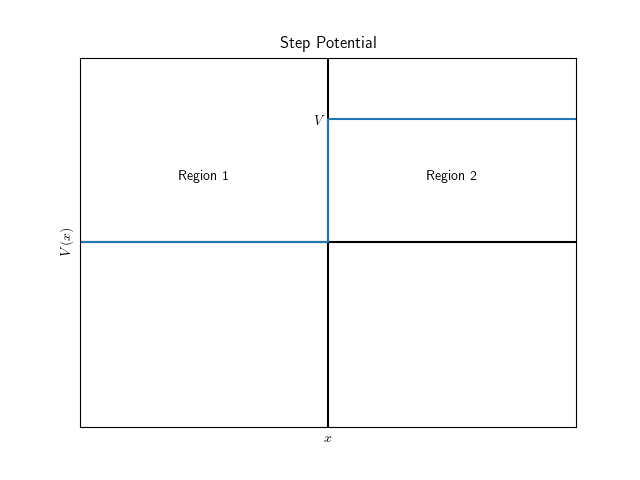
\includegraphics[scale=0.6]{step_potential.png}
        \caption{The step potential}
    \end{figure}
    
    \subsubsection{Case 1: \texorpdfstring{\(E > V\)}{E > V}}
    Classically we would expect a particle incident from the left with \(E > V\) to enter region 2, \(x > 0\).
    Since the total energy of the particle is constant and given by \(H = T + V\) then we would expect that upon entering region 2 the kinetic energy, and hence momentum, of the classical particle will have to decrease to keep the total energy constant.
    
    The \gls{tise} can be split into two section, in region 1, \(x < 0\), we have
    \[-\frac{\hbar^2}{2m}\dv[2]{x}\psi(x) = E\psi(x) \implies \psi''(x) = -\frac{p^2}{\hbar^2}\psi(x)\]
    where
    \[p = \sqrt{2mE},\]
    this is exactly the momentum of a classical particle with energy \(E\) and a potential energy of 0.
    In region 2 we have
    \[\left[-\frac{\hbar^2}{2m}\dv[2]{x}+ V\right]\psi(x) = E\psi(x) \implies \psi''(x) = -\frac{\bar{p}}{\hbar^2}\psi(x)\]
    where
    \[\bar{p} = \sqrt{2m(E - V)},\]
    this is exactly the momentum of a classical particle with energy \(E\) and a potential energy of \(V\).
    As we would expect the momentum in region 2, \(\bar{p}\), is less than the momentum in region 1, \(p\).
    Fortunately we already know the solution to the wave equation in both regions:
    \[
        \psi(x) =
        \begin{cases}
            Ae^{ipx/\hbar} + Be^{-ikp/\hbar}, &x < 0,\\
            Ce^{i\bar{p}x/\hbar} + De^{-i\bar{p}x/\hbar} &x > 0.
        \end{cases}
    \]
    The solutions are a superposition of waves with momentum \(\pm p\) and \(\pm\bar{p}\) in the respective region.
    By `wave with momentum \(p\)' we mean a wave function such that \(p\) is an eigenvalue of \(\operator{P}\).
    
    Suppose that a particle comes in from the left.
    Then we expect a wave propagating to the right in both regions and a wave propagating to the left in region 1 corresponding to the wave reflecting off the boundary.
    However there is no reason to expect a wave propagating left in region 2 as once the wave enters that region there is nothing to cause a reflection.
    Therefore \(D = 0\).
    
    We are left with three degrees of freedom, \(A\), \(B\), and \(C\).
    We can fix one by requiring a normalised wave function, say we choose \(A\) for this purpose.
    We then use the requirements of continuity of \(\psi\) and \(\psi'\) to fix the other two degrees of freedom.
    Clearly \(\psi\) and \(\psi'\) are continuous at all \(x \ne 0\) so we only need to consider continuity at \(x = 0\).
    We require that
    \[\lim_{x\to0^+}\psi(x) = \lim_{x\to0^-}\psi(x),\]
    and
    \[\lim_{x\to0^+}\psi'(x) = \lim_{x\to0^-}\psi'(x).\]
    The first of these gives us
    \[\lim_{x\to0^+}\psi(x) = \lim_{x\to0^+}\left[Ae^{ipx/\hbar} + Be^{-ikx/\hbar}\right] = A + B\]
    \[\lim_{x\to0^-}\psi(x) = \lim_{x\to0^-} Ce^{i\bar{p}x/\hbar} = C.\]
    Hence
    \[A + B = C.\]
    The second leads to 
    \[\lim_{x\to0^+}\psi'(x) = \lim_{x\to0^+}\left[\frac{ip}{\hbar}Ae^{ipx/\hbar} - \frac{ip}{\hbar}Be^{-ikx/\hbar}\right] = \frac{ip}{\hbar}A + \frac{ip}{\hbar}B\]
    \[\lim_{x\to0^-}\psi'(x) = \lim_{x\to0^-} \frac{i\bar{p}}{\hbar}Ce^{i\bar{p}x/\hbar} = \frac{i\bar{p}}{\hbar}C.\]
    Hence
    \[p(A + B) = \bar{p}C.\]
    We can then show that
    \[B = \frac{p - \bar{p}}{p + \bar{p}}A,\qquad\text{and}\qquad C = \frac{2p}{p + \bar{p}}A.\]
    This imposes no restrictions on the energy, \(E\) can take any value as long as it is greater than \(V\).
    The Hamiltonian has a continuous spectrum.
    Notice that in general \(B \ne 0\) so there is a reflected wave going left in region 1.
    
    \subsubsection{Case 2: \texorpdfstring{\(E < V\)}{E<V}}
    The situation is very similar if \(E < V\) but now region 2 is classically forbidden, meaning that a classical particle could not enter into this region.
    The equations for the wave function are the same but since \(E < V\) \(E - V\) is now negative meaning that \(\bar{p}\) is imaginary:
    \[\bar{p} = \sqrt{2m(E - V)} = i\sqrt{2m(V -  E)} = i\tilde{p}.\]
    In region 2 the solution to the wave function is now
    \[\psi(x) = Ce^{-\tilde{p}x/\hbar} + De^{\tilde{p}x/\hbar}.\]
    The first term is a decaying exponential and is finite in region 2.
    The second is an increasing exponential and therefore goes to infinity as \(x \to\infty\).
    This is not allowed so we discard this term in order for \(\psi\) to be normalisable.
    Hence in region 2
    \[\psi(x) = Ce^{-\tilde{p}x/\hbar}.\]
    Region 2 is classically forbidden but the wave function is non-zero in region 2 therefore there is a non-zero probability that the particle will be found in region 2.
    This time we can show that
    \[B = \frac{p - i\tilde{p}}{P + i\tilde{p}}A.\]
    The fraction here has unit modulus so we must have that \(\abs{B}^2 = \abs{A}^2\), this means that they just differ by a phase, \(\delta\):
    \[B = e^{-2i\delta(E)}A,\]
    here we emphasise the fact that \(\delta\) is a function of the energy (not the Dirac delta).
    It can also be shown that
    \[\tilde{p} = p\cot\delta.\]
    We define \(\lambda\) as the length that the particle penetrates the classically forbidden region and we note that it scales as \(\hbar/p\).
    
    \subsection{Potential Barrier}
    Consider the potential
    \[
        V(x) = 
        \begin{cases}
            V, & x \in [0, a],\\
            0, & x\notin[0, a],
        \end{cases}
    \]
    \begin{figure}[ht]
        \centering
        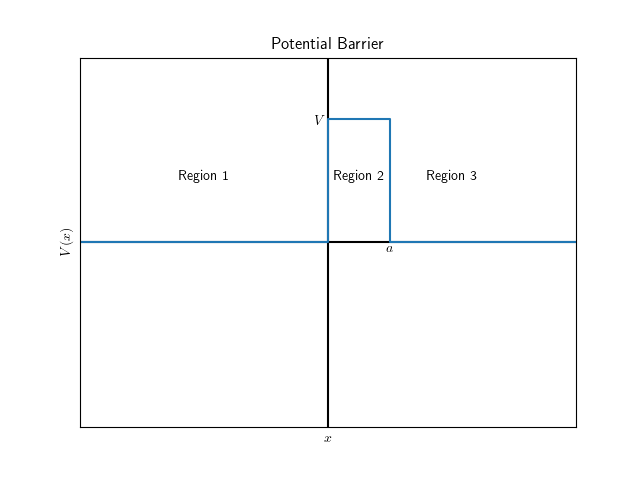
\includegraphics[scale=0.6]{potential_barrier.png}
        \caption{The potential barrier}
    \end{figure}
    for some positive constant, \(V\).
    Again there are two cases, \(E > V\) and \(E < V\).
    In the cases that \(E > V\) this is very similar to the same case with the potential step.
    The wave function will be oscillatory in all three regions with an amplitude that depends on the value of the potential.
    The interesting case is when \(E < V\).
    
    Classically when \(E < V\) region 2 is forbidden.
    A particle entering from the left has no way to go past the origin, it will reflect off the origin and go back to \(-\infty\).
    The solution to the Schr\"odinger equation is
    \[
        \psi(x) =
        \begin{cases}
            Ae^{ipx/\hbar} + Be^{ipx/\hbar}, & x \in (-\infty, 0),\\
            Ce^{-\tilde{p}x/\hbar} + De^{\tilde{p}x/\hbar}, &x \in (0, a),\\
            Fe^{ipx/\hbar} + Ge^{ipx/\hbar}, & x \in (a, \infty).
        \end{cases}
    \]
    Here \(p\) and \(\tilde{p}\) are defined as they were for the potential step.
    Notice that since \(x\) is finite in \((0, a)\) there is no reason to discard the term \(De^{\tilde{p}x/\hbar}\) as it is finite for all \(x\in(0, a)\).
    For the same reason as before if we have a particle coming in from the left we must have that \(G = 0\).
    So in region 3
    \[\psi(x) = Fe^{ipx/\hbar} = AS(E)e^{ip(x - a)/\hbar}.\]
    The last part of this is the conventional way to write this term.
    Of particular interest is \(S(E)\), this is the ratio of the probability amplitude of the wave entering the barrier at \(x = 0\), to the probability amplitude of the wave leaving the barrier at \(x = a\).
    \(S(E)\) can be shown to be
    \[S(E) = \frac{2ip\tilde{p}}{(p^2 - \tilde{p}^2)\sinh(\tilde{p}a/\hbar) + 2ip\tilde{p}\cosh(\tilde{p}a/\hbar)}.\]
    The transmissivity, \(T\), is defined as the probability that the particle tunnels through the barrier, that is
    \[T = \abs{S(E)}^2 = \left[1 + \frac{\sinh^2(\tilde{p}a/\hbar)}{4(E/V)(1 - E/V)}\right]^{-1}.\]
    For \(E < V\) this is a monotonically increasing function of \(E\) for a fixed value of \(a\).
    This means that as the energy increases the probability that the particle tunnels through the barrier increases.
    Importantly
    \[T \propto e^{-ka}\]
    for some constant \(k\).
    Therefore as \(a\) increases for a fixed value of \(E\) the probability that the particle tunnels into region 3 decreases.
    
    \subsubsection{Tunnelling}
    Tunnelling is a phenomenon without classical analogue.
    It can be experimentally verified and is one of many confirmations that quantum mechanics yields correct predictions.
    Tunnelling has many applications in physics.
    
    The process of alpha decay can be seen as a process of the alpha particle tunnelling out of a potential well created by the nucleus.
    Figure~\ref{fig:alpha decay} shows a phenomenological potential used to model alpha decay.
    The alpha particle is in a potential well and typically has less energy than the maximum potential.
    However it is still possible for the alpha particle to tunnel out of the well, and out of the nucleus.
    \begin{figure}[ht]
        \centering
        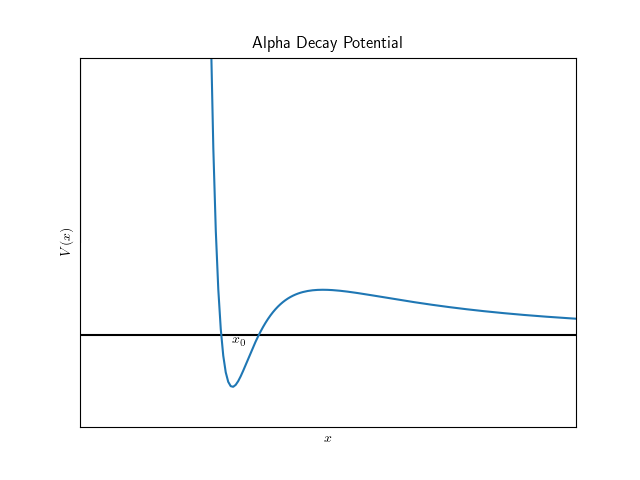
\includegraphics[scale=0.6]{alpha_decay.png}
        \caption{The potential modelling the alpha decay process. An alpha particle in the nucleus is in the potential well at \(x_0\), it can then tunnel outside of this well to some positive \(x\) value even if it has less energy than the peak on the right of the potential well.}
        \label{fig:alpha decay}
    \end{figure}

    \subsubsection{Scanning Tunnelling Microscope}
    A \gls{stm} is made of a needle that is placed near the surface of a material.
    A current of electrons is applied to the needle.
    We can model the air gap between the needle point and the surface as a potential barrier.
    The electrons tunnel across this gap and a current flows.
    The current is proportional to the probability of an electron tunnelling so
    \[I \propto e^{-ka}.\]
    This allows for very small changes in the size of the air gap to be measured accurately by measuring the current.
    Scanning the \gls{stm} over the whole surface we can build up a picture of the 3-dimensional structure of the surface.
    
    \subsection{Infinite Potential Well}\label{sec:infinite square well}
    An infinite potential well of width \(a\) is a potential,
    \[
        V(x) =
        \begin{cases}
            0, & x \in(-a/2, a/2)\\
            \infty, & x\notin (-a/2, a/2).
        \end{cases}
    \]
    We are looking for the solutions to the \gls{tise} with positive energy (as the minimum potential is zero and the energy must be at least as large as this).
    We can view each boundary at \(\pm a/2\) as a potential step and then let \(V\to\infty\).
    The solution in these regions is
    \[\psi \sim e^{-\tilde{p}\delta/\hbar}.\]
    For finite \(V\)
    \[\tilde{p} = \sqrt{2m(V - E)}.\]
    As \(V\to\infty\) \(\tilde{p} \to \infty\) and so \(\psi\to 0\).
    We see that the regions outside of the well are not only classically forbidden but completely inaccessible, even to a quantum particle.
    
    Therefore we only need to solve the \gls{tise} in the region \((-a/2, a/2)\) and apply boundary conditions at \(x = \pm a/2\).
    The boundary conditions here are \(\psi(\pm a/2) = 0\) as we require continuity of \(\psi\).
    Note that since \(V\) is not finite we do not require continuity of \(\psi'\).
    The general form of the solution in the well is that of a free particle:
    \[\psi(x) = Ae^{ikx} + Be^{-ikx}\]
    where \(k = p/\hbar\) and \(p = \sqrt{2mE}\) is the classical momentum.
    At the boundaries we have
    \[\psi(a/2) = Ae^{ika/2} + Be^{-ika/2} = 0 \implies B = -Ae^{ika},\]
    substituting this into the second boundary condition we have
    \begin{align*}
        \psi(-a/2) &= Ae^{-ika/2} - Ae^{ika}e^{ika/2}\\
        &= Ae^{ika/2}(e^{-ika} - e^{ika})\\
        &= Ae^{ika/2}[\cos(ka) - i\sin(ka) - \cos(ka) - i\sin(ka)]\\
        &= 2iAe^{ika/2}\sin(ka).
    \end{align*}
    We require this to be zero.
    Since \(2iAe^{ika/2}\ne 0\) (assuming \(A\) is non-zero, as it must be for any wave function of interest) we must have that \(\sin(ka) = 0\).
    Therefore
    \[ka = n\pi \implies k = \frac{n\pi}{a},\qquad n\in\naturals.\]
    From this we have
    \[\frac{n\pi}{a} = k = \frac{p}{\hbar} = \frac{\sqrt{2mE}}{\hbar} \implies E = \frac{n^2\pi^2\hbar^2}{2ma^2}.\]
    Since \(n\in\naturals\) the energy, \(E\), is quantised.
    From now on we will denote the energy of the \(n\)th state as
    \[E_n = \frac{1}{2m}\left(\frac{\hbar\pi n}{a}\right)^2.\]
    If we normalise the wave functions we find that the properly normalised eigenstates of the Hamiltonian are
    \[
        u_n =
        \begin{cases}
            \sqrt{\frac{2}{a}}\sin\left(\frac{n\pi x}{a}\right), & n~\text{even},\\
            \sqrt{\frac{2}{a}}\cos\left(\frac{n\pi x}{a}\right), & n~\text{odd}.
        \end{cases}
    \]
    Since \(u_n(x) = 0\) is boring we consider \(u_1\) to be the ground state.
    In this state the particle is most likely to be found at \(x = 0\).
    The first four wave functions, and the associated probability densities, are shown in figure~\ref{fig:infinite square well wave functions}.
    \begin{figure}[ht]
        \centering
        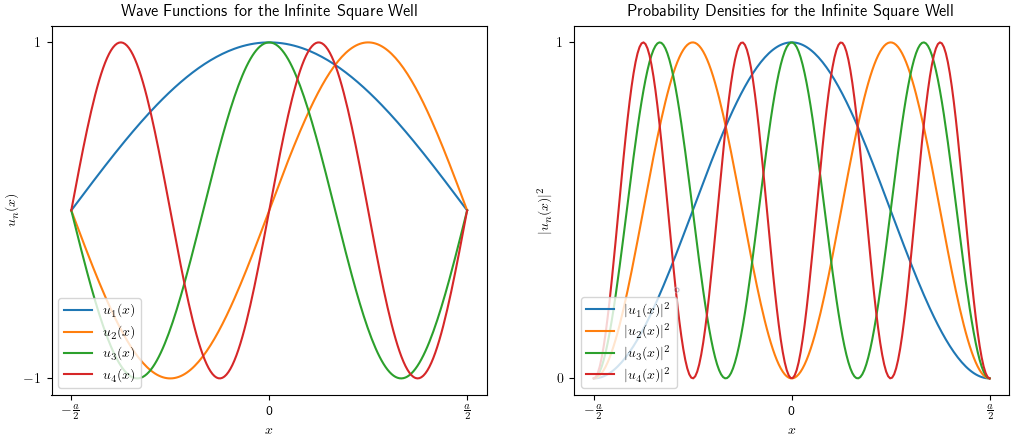
\includegraphics[scale=0.5]{infinite_square_well_wave_func.png}
        \caption{The first four wave functions, \(u_n\), for the infinite square well and the the associated probability densities.}
        \label{fig:infinite square well wave functions}
    \end{figure}
    The generic state of a particle in an infinite square well potential is a linear combination of \(\{u_n(x)\}\).
    That is a linear superposition of eigenstates of \(\operator{P}\) with eigenvalues
    \[\pm p_n = \pm \hbar k_n = \pm\frac{n\pi\hbar}{a}.\]
    
    \subsubsection{Zero Point Energy}
    Notice that in the ground state \(p_1 = \pi\hbar/a \ne 0\).
    This can be seen as a direct consequence of \gls{hup}.
    Since the particle is constrained to have \(x\in(-a/2, a/2)\) this gives us a maximum uncertainty in \(x\) of \(\Delta x = a\).
    Hence
    \[\Delta p\Delta x \ge \frac{\hbar}{2} \implies \Delta p \ge \frac{\hbar}{2a}.\]
    Therefore the momentum cannot be zero, as then we would know the value with zero uncertainty, which is certainly less than \(\hbar/2a\).
    The energy in this state is consequently also non-zero:
    \[E \sim \frac{(\Delta p)^2}{2m} \ge \frac{\hbar^2}{8ma}.\]
    The kinetic energy due to the uncertainty principle is called the zero point energy.
    One consequence of this is that helium can be a liquid at \(T = \SI{0}{\kelvin}\).
    This is because in order to form a solid the atoms must be constrained to a lattice giving them some non-zero zero point energy, which scales inversely to the mass, for a particle as light as helium it is enough to overcome interatomic forces and the system remains in a liquid phase.
    
    \subsubsection{Symmetry of the Solutions}
    The energy eigenstates have definite parity, that is if we define the parity operator, \(\operator{\parity}\), to have the action
    \[\operator{\parity}\psi(x) = \psi(-x),\]
    then the energy eigenstates are also eigenstates of the parity operator:
    \[\operator{\parity}u_n(x) = (-1)^{n+1}u_n(x).\]
    This can be seen from the explicit form of \(u_n\) and using the fact that sine and cosine are odd and even functions respectively.
    This means that \(u_n\) are simultaneously eigenfunctions of \(\operator{\parity}\), \(\operator{P}\), and \(\operator{H}\).
    
    We can show that in general if the potential is symmetric, so \(V(-x) = V(x)\), then \([\operator{H}, \operator{\parity}] = 0\), that is \(\operator{H}\) is symmetric under \(\operator{\parity}\).
    This then implies the existence of a basis of simultaneous eigenstates of \(\operator{H}\) and \(\operator{\parity}\).
    
    It is fairly simple to show the above paragraph is true.
    Suppose that \(V\) is a symmetric potential.
    Then
    \begin{align*}
        \operator{\parity}\operator{H}\psi(x) &= \operator{\parity}\left[-\frac{\hbar^2}{2m}\dv[2]{x} + V(x)\right]\psi(x)\\
        &= \operator{\parity}\left[-\frac{-\hbar^2}{2m}\dv[2]{\psi(x)}{x} + V(x)\psi(x)\right]\\
        &= -\frac{\hbar^2}{2m}\dv[2]{\psi(-x)}{x} + V(-x)\psi(-x)\\
        &= -\frac{\hbar^2}{2m}\dv[2]{\psi(-x)}{x} + V(x)\psi(-x).
     \end{align*}
    Here we have used the fact that
    \[\operator{\parity}\dv{x} = \dv{-x} = -\dv{x}\]
    and hence
    \[\operator{\parity}\dv[2]{x} = -\dv{x}\left(-\dv{x}\right) = \dv[2]{x}.\]
    Also
    \begin{align*}
        \operator{H}\operator{\parity}\psi(x)& = \operator{H}\psi(-x)\\
        &= \left[-\frac{\hbar^2}{2m}\dv[2]{x} + V(x)\right]\psi(-x)\\
        &= -\frac{\hbar^2}{2m}\dv[2]{\psi(-x)}{x} + V(x)\psi(-x).
    \end{align*}
    Hence
    \[[\operator{\parity}, \operator{H}] = 0.\]
    We know that this means there is a common basis of eigenstates but how do we find it?
    The states
    \[v_n^+(x) = u_n(x) + u_n(-x),\qquad\text{and}\qquad v_n^-(x) = u_n(x) - u_n(-x)\]
    are one such basis.
    These states can be compactly written as
    \[v_n^{\pm}(x) = (1 \pm \operator{\parity})u_n(x).\]
    It is then easy to show that these are eigenstates of \(\operator{H}\) and \(\operator{\parity}\):
    \begin{multline*}
        \operator{H}v_n^{\pm}(x) 
        = \operator{H}(1 \pm \operator{\parity})u_n(x) 
        = \operator{H}u_n(x) \pm \operator{H}\operator{\parity}u_n(x) 
        = \operator{H}u_n(x) \pm \operator{\parity}\operator{H}u_n(x) \\
        = E_nu_n(x) + E_n\operator{\parity}u_n(x) 
        = E_n(1 \pm \operator{\parity})u_n 
        = E_nv_n^{\pm}(x).
    \end{multline*}
    and
    \begin{multline*}
        \operator{\parity}v_n^{\pm}(x) 
        = \operator{\parity}(1 \pm \operator{\parity})u_n(x)
        = \operator{\parity}u_n(x) \pm \operator{\parity}^2u_n(x)
        = \operator{\parity}u_n(x) \pm (-1)^{n+1}(-1)^{n+1}u_n(x)\\ 
        = \operator{\parity}u_n(x) \pm u_n(x)
        = \operator{\parity}u_n(x) \pm u_n(x)
        = \pm(1 \pm \operator{\parity})u_n(x)
    \end{multline*}

    \subsection{Finite Potential Well}
    The finite potential well has the potential
    \[
        V(x) = 
        \begin{cases}
            -V_0, & x\int(-a/2, a/2),\\
            0, & x\notin(-a/2, a/2),
        \end{cases}
    \]
    for some positive constant \(V_0\).
    This potential is symmetric under parity change.
    This means that we can look for a set of energy eigenstates that are also parity eigenstates.
    The energy eigenvalues must be greater than \(-V_0\).
    States with \(-V_0 < E < 0\) are called \define{bound states}.
    The wave function for these states decays exponentially for \(\abs{x} > a/2\) so the probability of finding the particle outside of the well becomes small quickly.
    The states with \(E > 0\) are simply plane waves that have a momentum change and chance of reflection at each boundary, this isn't that interesting and is just like the potential step so we won't consider these states further.
    
    The Schr\"odinger equation is
    \[
        \psi''(x) = 
        \begin{cases}
            -\frac{2m}{\hbar^2}E\psi(x), & \abs{x} > a/2,\\
            -\frac{2m}{\hbar^2}(E + V_0)\psi(x), & \abs{x} < a/2.
        \end{cases}
    \]
    Unlike the infinite well the wave function is non-zero outside the well.
    For \(-V_0 < E < 0\) the even parity solutions are
    \[
        \psi(x) =
        \begin{cases}
           A\cos(px/\hbar), & \abs{x} < a/2,\\
           Ce^{-\bar{p}x/\hbar}, & x > a/2,\\
           Ce^{\bar{p}x/\hbar}, & x < -a/2.
        \end{cases}
    \]
    The odd parity solutions are
    \[
        \psi(x) =
        \begin{cases}
            A\sin(px/\hbar), & \abs{x} < a/2,\\
            Ce^{-\bar{p}x/\hbar}, & x > a/2,\\
            -Ce^{\bar{p}x/\hbar}, & x < -a/2.
        \end{cases}
    \]
    We have introduced the momenta
    \[p = \sqrt{2m(E + V_0)},\qquad\text{and}\qquad \bar{p}\sqrt{-2mE}.\]
    There are two things to notice here, first \(-V_0 < E < 0\) so \(p, \bar{p}\in\reals\), and here the factor of \((E + V_0)\) appears in \(p\) whereas previously it appeared in \(\bar{p}\).
    The reason for this is that previously we viewed the minimum of the potential as \(0\) and the maximum as \(V\) but here the minimum is \(-V_0\) and the maximum is \(0\).
    
    Imposing continuity at \(a/2\) in both the wave function and its derivative we have for the even solutions that
    \begin{align*}
        A\cos\left(\frac{pa}{2\hbar}\right) &= Ce^{-\bar{p}a/2\hbar}\\
        -\frac{p}{\hbar}A\sin\left(\frac{pa}{2\hbar}\right) &= -\frac{\bar{p}a}{\hbar}Ce^{-\bar{p}a/2\hbar}.
    \end{align*}
    Dividing the first equation by the second we get the quantisation condition
    \[p\tan\left(\frac{pa}{2\hbar}\right) = \bar{p}.\]
    Similarly for the odd parity solutions we have
    \begin{align*}
        A\sin\left(\frac{pa}{2\hbar}\right) &= Ce^{-\bar{p}a/2\hbar}\\
        \frac{p}{\hbar}A\cos\left(\frac{pa}{2\hbar}\right) &= -\frac{\bar{p}a}{\hbar}Ce^{-\bar{p}a/2\hbar}.
    \end{align*}
    This leads to
    \[p\cot\left(\frac{pa}{2\hbar}\right) = -\bar{p}.\]
    There is always at least one even bound state.
    For small \(V_0\), corresponding to a shallow well, it can be shown that
    \[E = -\frac{mV_0^2a^2}{2\hbar^2}\]
    for the ground state.
    
    \section{Harmonic Oscillators}
    \subsection{The Classical Harmonic Oscillators}
    The equation of motion for a classical particle of mass \(m\) undergoing one-dimensional harmonic oscillations, undergoing a restoring force proportional to the displacement, is
    \[m\ddot{x} = -kx.\]
    The constant \(k\) is often called the spring constant due to the common example of a mass on a spring where this is exactly what \(k\) is.
    The solution is oscillatory with an angular frequency
    \[\omega = \sqrt{\frac{k}{m}}.\]
    Using the chain rule we have
    \[\ddot{x} = \dv[2]{x}{t} = \dv{v}{t} = \dv{v}{x}\dv{x}{t} = v\dv{v}{x}.\]
    Integrating the equation of motion we then have
    \[m\int v\dv{v}{x}\dd{x} = -k\int x\dd{x} \implies \frac{1}{2}mv^2 = -\frac{1}{2}kx^2 + E\]
    where \(E\) is the total energy of the system, which appears as a constant of integration.
    Thus
    \[\frac{1}{2}mv^2 + \frac{1}{2}kx^2 = E.\]
    Identifying the first term as the kinetic energy we see that the potential energy is
    \[V(x) = \frac{1}{2}kx^2 = \frac{1}{2}m\omega^2x^2.\]
    The total energy is
    \[E = \frac{1}{2}m\omega^2L^2\]
    where \(L\) is the amplitude of the oscillations.
    It is easy to show that this is the maximum energy by noting that at \(x = L\) the particle is instantaneously stationary as it changes direction so the kinetic energy is zero.
    
    \subsection{The Quantum Harmonic Oscillator}
    The transformation to the quantum case is straight forward.
    The potential is simply
    \[V(\operator{X}) = \frac{1}{2}m\omega^2\operator{X}^2.\]
    Assuming a discrete spectrum we have to solve the \gls{tise}:
    \[\operator{H}\ket{n} = E_n\ket{n},\]
    where
    \[\operator{H} = \frac{\operator{P}^2}{2m} + \frac{1}{2}m\omega^2\operator{X}^2.\]
    Taking the inner product of the \gls{tise} with an eigenstate of \(\operator{X}\) we have
    \[\bra{x}\operator{H}\ket{n} = E_n\braket{x}{n} = E_nu_n(x)\]
    defining \(u_n(x) = \braket{x}{n}\) as the energy eigenfunction with energy \(E_n\).
    The full \gls{tise} is then
    \[\left[-\frac{\hbar^2}{2m}\dv[2]{x} + \frac{1}{2}m\omega^2 x^2\right]u_n(x) = E_nu_n(x).\]
    
    \subsection{The Solutions to the Harmonic Oscillator}
    We will start by discussing the solutions to this and look at deriving them in later sections.
    The first thing to note is that the energy is quantised as follows:
    \[E_n = \left(n + \frac{1}{2}\right)\hbar\omega,\qquad\text{where}\qquad n\in\naturals.\]
    The ground state corresponds to \(n = 0\) and has the non-zero energy \(E_0 = \hbar\omega/2\).
    The energy eigenfunctions are
    \[u_n(x) = C_ne^{-\alpha^2x^2/2}H_n(\alpha x).\]
    Here \(C_n\) is a normalisation constant, \(\alpha^2 = m\omega/\hbar\) and \(H_n\) are polynomials of degree \(n\) called the \define{Hermite polynomials}.
    The Hermite polynomials are orthogonal in such that
    \[\int_{-\infty}^{\infty} \dd{s}e^{-s^2}H_m(s)H_n(s) = 2^n\sqrt{\pi}n!\delta_{mn},\]
    which is only non-zero if \(n = m\).
    The first four Hermite polynomials are
    \begin{align*}
        H_0(s) &= 1,  & H_2(s) &= 4s^2 - 2,\\
        H_1(x) &= 2s, & H_3(s) &= 8s^3 - 12s.
    \end{align*}
    Note that if \(n\) is even (odd) then \(H_n(s)\) only contains even (odd) powers of \(s\), this is true for all \(n\).
    This means that the Hermite polynomials have even (odd) parity for even (odd) \(n\).
    Since the Gaussian term of \(u_n\) has even parity this means that the parity of \(u_n\) is the same as \(H_n\).
    That is
    \[\operator{\parity}u_n(x) = u_n(-x) = (-1)^nu_n(x).\]
    We see that the energy eigenstates are eigenstates of the parity operator, \(\operator{\parity}\), which is a direct consequence of the potential being symmetric:
    \[V(-x) = \frac{1}{2}m\omega^2(-x)^2 = \frac{1}{2}m\omega^2x^2 = V(x).\]
    Since \(u_n\) has definite parity \(\abs{u_n(x)}^2\) is even.
    Therefore
    \[\expected{x}_n = \bra{n}\operator{X}\ket{n} = \int_{-\infty}^{\infty} \dd{x} x\abs{u_n(x)}^2 = 0,\]
    as the integrand is always odd and an integral of an odd function over an even interval, \((-\infty, \infty)\), is zero.
    Strictly speaking this only holds if the integral converges but in this case it clearly does as the Gaussian part goes to zero much faster than the polynomial parts can go to infinity.
    A quick sanity check here would be to think about the potential and since it is symmetric the particle is equally likely to be at a positive \(x\) as it is at a negative \(x\) and therefore the expected value should be zero.
    
    The next quantity that we might want to compute is the expected value of \(x^2\) which is
    \[\expected{x^2}_n = \int_{-\infty}^{\infty} \dd{x} x^2\abs{u_n(x)}^2 = \left(n + \frac{1}{2}\right)\frac{1}{\alpha^2}.\]
    From this we can see that for larger energies it becomes more probable to find the particle at large \(x\), that is the variance, \(\Delta x_n = \expected{x}_n - \expected{x}_n^2 = \expected{x^2}_n\), increases with energy:
    \[E_n = m\omega^2\expected{x^2}_n.\]
    Compare this to the classical energy,
    \[E = \frac{1}{2}m\omega^2L^2.\]
    
    \subsection{Solving the Harmonic Oscillator (The Fancy Way)}
    \subsubsection{Factorising the Hamiltonian}
    The Hamiltonian is
    \[\operator{H} = \frac{\operator{P}^2}{2m} + \frac{1}{2}m\omega^2\operator{X}^2.\]
    We can factor out \(\hbar\omega\) from this:
    \[\operator{H} = \hbar\omega\left[\frac{1}{2m\hbar\omega}\operator{P}^2 + \frac{m\omega}{2\hbar}\operator{X}^2 \right].\]
    Since \(\hbar\omega\) has units of energy the term in the brackets must be dimensionless.
    We define two operators
    \[\operator{\xi} = \sqrt{\frac{m\omega}{2\hbar}}, \qquad\text{and}\qquad \operator{\eta} = \frac{1}{\sqrt{2m\hbar\omega}}\operator{P}.\]
    These are simply rescaled, dimensionless, versions of the position and momentum operators.
    The Hamiltonian can now be written as
    \[\operator{H} = \hbar\omega[\operator{\xi}^2 + \operator{\eta}^2].\]
    Since \(\operator{\xi}\) and \(\operator{\eta}\) are proportional to the position and momentum operators we know that they don't commute, in fact their commutator is
    \begin{align*}
        [\operator{\xi}, \operator{\eta}] &= \sqrt{\frac{m\omega}{2\hbar}}\frac{1}{\sqrt{2m\hbar\omega}} [\operator{X}, \operator{P}]\\
        &= \frac{1}{2\hbar}[\operator{X}, \operator{P}]\\
        &= \frac{i}{2}.
    \end{align*}
    There are two checks that it is good to do here.
    First since \(\operator{\xi}\) and \(\operator{\eta}\) are dimensionless their commutator should be too, and it is.
    Second since \(\operator{X}\) and \(\operator{P}\) are Hermitian then so are \(\operator{\xi}\) and \(\operator{\eta}\) and therefore their commutator should be anti-Hermitian, and it is.
    
    We now define a new operator:
    \[\operator{a} = \operator{\xi} + i\operator{\eta},\qquad\text{and}\qquad \operator{a}\hermit = \operator{\xi} - i\operator{\eta}.\]
    The motivation behind this is that if \(\operator{\xi}\) and \(\operator{\eta}\) commuted then we could factorise the Hamiltonian as
    \[\hbar\omega(\operator{\xi} + i\operator{\eta})(\operator{\xi} - i\operator{\eta}).\]
    However we cannot do this.
    We can write this new operator in terms of \(\operator{X}\) and \(\operator{P}\):
    \begin{align*}
        \operator{a} &= \sqrt{\frac{m\omega}{2\hbar}} \operator{X} + \frac{i}{\sqrt{2m\omega\hbar}} \operator{P} = \sqrt{\frac{m\omega}{2\hbar}}\left[\operator{X} + \frac{i}{m\omega}\operator{P}\right]\\
        \operator{a}\hermit &= \sqrt{\frac{m\omega}{2\hbar}} \operator{X} - \frac{i}{\sqrt{2m\omega\hbar}} \operator{P} = \sqrt{\frac{m\omega}{2\hbar}}\left[\operator{X} - \frac{i}{m\omega}\operator{P}\right]\\
    \end{align*}
    We can then compute
    \begin{align*}
        \operator{a}\operator{a}\hermit &= (\operator{\xi} + i\operator{\eta})(\operator{\xi} - i\operator{\eta})\\
        &= \operator{\xi}^2 + i\operator{\eta}\operator{\xi} - i\operator{\xi}\operator{\eta} + \operator{\eta}^2\\
        &= \operator{\xi} + i[\operator{\eta}, \operator{\xi}] + \operator{\eta}^2,
    \end{align*}
    and
    \begin{align*}
        \operator{a}\hermit\operator{a} &= (\operator{\xi} - i\operator{\eta})(\operator{\xi} + i\operator{\eta})\\
        &= \operator{\xi}^2 + i\operator{\xi}\operator{\eta} - i\operator{\eta}\operator{\xi} + \operator{\eta}^2\\
        &= \operator{\xi}^2 - i[\operator{\eta}, \operator{\xi}] + \operator{\eta}^2.
    \end{align*}
    Subtracting these two equations we have
    \[[\operator{a}, \operator{a}\hermit] = 1,\]
    and adding the equations we have
    \[\operator{H} = \frac{1}{2}\hbar\omega(\operator{a}\operator{a}\hermit + \operator{a}\hermit\operator{a}).\]
    A more useful form for the Hamiltonian can be found by adding zero:
    \[\operator{H} = \frac{1}{2}\hbar\omega(\operator{a}\operator{a}\hermit + \operator{a}\hermit\operator{a}) = \frac{1}{2}\hbar\omega(\operator{a}\operator{a}\hermit - \operator{a}\hermit\operator{a} + \operator{a}\hermit\operator{a}+ \operator{a}\hermit\operator{a}) = \frac{1}{2}\hbar\omega([\operator{a}, \operator{a}\hermit] + 2\operator{a}\hermit\operator{a}) = \hbar\omega\left(\operator{a}\hermit\operator{a} + \frac{1}{2}\right).\]
    
    \subsubsection{Creation and Annihilation}
    For this section we will need the commutators of \(\operator{a}\) and \(\operator{a}\hermit\) with the Hamiltonian, fortunately these are fairly easy to compute now:
    \[[\operator{H}, \operator{a}] = \left[\hbar\omega\left(\operator{a}\hermit \operator{a} + \frac{1}{2}\right), \operator{a}\right] = \hbar\omega[\operator{a}\hermit\operator{a}, \operator{a}]\]
    using the fact that \([1/2, \operator{a}] = 0\).
    Then
    \[[\operator{a}\hermit\operator{a}, \operator{a}] = \operator{\hermit}\operator{a}\operator{a} - \operator{a}\operator{a}\hermit\operator{a} = [\operator{a}\hermit, \operator{a}]\operator{a} = -\operator{a}.\]
    Therefore
    \[[\operator{H}, \operator{a}] = \hbar\omega [\operator{a}\hermit\operator{a}, \operator{a}] = -\hbar\omega\operator{a.}\]
    Similarly
    \[[\operator{H}, \operator{a}\hermit] = \left[\hbar\omega\left(\operator{a}\hermit \operator{a} + \frac{1}{2}\right), \operator{a}\hermit\right] = \hbar\omega[\operator{a}\hermit\operator{a}, \operator{a}\hermit] = \hbar\omega(\operator{a}\hermit\operator{a}\operator{a}\hermit - \operator{a}\hermit\operator{a}\hermit\operator{a}) = \hbar\omega\operator{a}\hermit[\operator{a}, \operator{a}\hermit] = \hbar\omega\operator{a}\hermit.\]
    Suppose \(\ket{n}\) is an energy eigenstate.
    We would like to know how \(\operator{a}\) acts on this since working in the energy eigenbasis we can then describe the action of \(\operator{a}\) on any state.
    To do this we will use that
    \[\operator{H}\operator{a} = \operator{a}\operator{H} + \operator{H}\operator{a} - \operator{a}\operator{H} = \operator{a}\operator{H} + [\operator{H}, \operator{a}].\]
    Thus
    \begin{align*}
        \operator{H}(\operator{a}\ket{n}) &= \operator{a}\operator{H}\ket{n} + [\operator{H}, \operator{a}]\ket{n}\\
        &= E_n\operator{a}\ket{n} - \hbar\omega\operator{a}\ket{n}\\
        &= (E_n - \hbar\omega)\operator{a}\ket{n}.
    \end{align*}
    So we see that \(\operator{a}\ket{n}\) is another eigenstate of \(\operator{H}\) with energy \(E_n - \hbar\omega\), unless \(\operator{a}\ket{n} = 0\).
    For this reason we say that \(\operator{a}\) is a \define{lowering operator} as its action is to return an eigenstate of lower energy.
    It is also called an \define{annihilation operator} as it annihilates one quantum of energy, \(\hbar\omega\), from the system.\footnote{\(\operator{a}\) and \(\operator{a}\hermit\) don't correspond to physical processes so we don't need to consider energy conservation.}
    Similarly
    \begin{align*}
        \operator{H}(\operator{a}\dagger\ket{n}) &= \operator{a}\operator{H}\ket{n} + [\operator{H}, \operator{a}\hermit]\\
        &= E_n\operator{a}\ket{n} + \hbar\omega\operator{a}\hermit\\
        &= (E_n + \hbar\omega)\operator{a}\hermit\ket{n}.
    \end{align*}
    So again \(\operator{a}\hermit\ket{n}\) is an energy eigenstate, this time with higher energy \(E_n + \hbar\omega\).
    We call \(\operator{a}\hermit\) a \define{raising operator} as its action is to return an eigenstate of higher energy.
    It is also called a \define{creation operator} as it adds one quantum of energy, \(\hbar\omega\), to the system.
    
    If \(\ket{n}\) is an energy eigenstate with energy \(E_n\) then define \(\ket{n\pm 1}\) to be an energy eigenstate with energy \(E_n \pm \hbar\omega\).
    Then
    \[\operator{a}\ket{n} = c_n\ket{n - 1},\qquad\text{and}\qquad \operator{a}\hermit\ket{n} = d_n\ket{n + 1}.\]
    Here \(c_n\) and \(d_n\) are constants of proportionality and not eigenvalues.
    
    By successive application of the annihilation operator, \(\operator{a}\), we can get states with lower and lower energy unless at some point \(\operator{a}\ket{0} = 0\) we call the state \(\ket{0}\) the ground state.
    Such a state must exist as the potential is bounded below and the energy is always at least as large as the minimum of the potential.
    We can find the ground state energy by applying the Hamiltonian:
    \[\operator{H}\ket{0} = \hbar\omega \left(\operator{a}\hermit\operator{a} + \frac{1}{2}\right)\ket{0} =  \hbar\omega\operator{a}\hermit\underbrace{\operator{a}\ket{0}}_{=0}\frac{\hbar\omega}{2}\ket{0} = \frac{\hbar\omega}{2}\ket{0}\]
    so we see that the ground state of the Harmonic oscillator has energy \(\hbar\omega/2\).
    
    Going the other way we can start from the ground state and construct states with progressively higher and higher energies by applying the creation operator, \(\operator{a}\hermit\).
    Unlike with the annihilation operator there is no reason that this should ever yield zero as the energy is in theory unbounded above.
    The first application of the creation operator gives
    \[\operator{a}\hermit \ket{0} = d_0\ket{1}\]
    where \(\ket{1}\) is a state with energy
    \[E_1 = \hbar\omega\left(1 + \frac{1}{2}\right) = \frac{3}{2}\hbar\omega.\]
    A second application gives
    \[\operator{a}\hermit{^2}\ket{0} = d_0\operator{a}\hermit\ket{1} = d_0d_1\ket{2}.\]
    At this point we see that we really need to know what \(c_n\) and \(d_n\) are.
    We find them by considering the expectation values of \(\operator{a}\hermit\operator{a}\) and \(\operator{a}\operator{a}\hermit\) and requiring all states be normalised:
    \begin{align*}
        \bra{n}\operator{a}\hermit\operator{a}\ket{n} &= c_n\bra{n}\operator{a}\hermit\ket{n - 1}\\
        &= c_n\bra{n-1}\operator{a}\ket{n}^*\\
        &= c_nc_n^*\braket{n-1}{n-1}\\
        &= \abs{c_n}^2.
    \end{align*}
    Also
    \[\operator{a}\hermit\operator{a} = \frac{1}{\hbar\omega}\operator{H} - \frac{1}{2}\]
    so
    \begin{align*}
        \bra{n}\operator{a}\hermit\operator{a}\ket{n} &= \frac{1}{\hbar\omega}\bra{n}\operator{H}\ket{n} - \frac{1}{2}\braket{n}{n}\\
        &= \frac{1}{\hbar\omega}E_n\braket{n}{n} - \frac{1}{2}\braket{n}{n}\\
        &= \frac{1}{\hbar\omega}\left(n + \frac{1}{2}\right)\hbar\omega  - \frac{1}{2}\\
        &= n
    \end{align*}
    Since states are only defined up to a phase factor we are free to choose \(c_n\) to be a real, positive, number so
    \[c_n = \sqrt{n}.\]
    For \(d_n\) consider
    \begin{align*}
        \bra{n}\operator{a}\operator{a}\hermit\ket{n} &= d_n \bra{n}\operator{a}\ket{n + 1}\\
        &= d_n\bra{n + 1}\operator{a}\hermit\ket{n}^*\\
        &= d_nd_n^*\braket{n + 1}{n + 1}
    \end{align*}
    Also
    \[\operator{a}\operator{a}\hermit = \frac{1}{\hbar\omega}\operator{H} + \frac{1}{2}\]
    so
    \begin{align*}
        \bra{n}\operator{a}\operator{a}\hermit\ket{n} &= \frac{1}{\hbar\omega}\bra{n}\operator{H}\ket{n} + \frac{1}{2}\braket{n}{n}\\
        &= \frac{1}{\hbar\omega}E_n\braket{n}{n} + \frac{1}{2}\braket{n}{n}\\
        &= \frac{1}{\hbar\omega}\left(n + \frac{1}{2}\right)\hbar\omega + \frac{1}{2}\\
        &= n + 1.
    \end{align*}
    So, again choosing \(d_n\) to be real and positive, we have
    \[d_n = \sqrt{n + 1}.\]
    So the full action of the raising and lowering operators is
    \[\operator{a}\ket{n} = \sqrt{n}\ket{n - 1},\qquad\text{and}\qquad \operator{a}\hermit\ket{n} = \sqrt{n + 1}\ket{n + 1}.\]
    We see that the action of \(\operator{a}\) on the ground state is
    \[\bra{x}\operator{a}\ket{0} = \bra{x}\sqrt{0}\ket{?} = 0\]
    for all \(\ket{x}\), as expected.
    
    \subsubsection{The Wave Function}
    We have introduced these creation and annihilation operators but we have yet to show that they allow us to find the correct wave functions for the system.
    We define \(\braket{x}{n} = u_n(x)\) and also we know for the ground state that \(\bra{x}\operator{a}\ket{0} = \operator{a}u_0(x) = 0\).
    We can also expand this with the definition of \(\operator{a}\) in terms of position and momentum operators:
    \begin{align*}
        0 &= \operator{a}u_0(x)\\
        &= \sqrt{\frac{m\omega}{2\hbar}}\left[\operator{X} + \frac{i}{m\omega}\operator{P}\right]u_0(x)\\
        &= \sqrt{\frac{m\omega}{2\hbar}}\left[x - \frac{i}{m\omega}i\hbar\dv{x}\right]u_0(x)\\
        \implies 0 &= xu_0(x) + \frac{\hbar}{m\omega}\dv{u_0}{x}\\
        \implies \dv{u_0}{x} &= -\frac{m\omega}{\hbar}xu_0(x)\\
        &= \alpha^2xu_0(x)\\
        \implies \frac{1}{u_0}\dv{u_0}{x} &= -\alpha x\\
        \implies \int \frac{1}{u_0}\dd{u_0} &= -\alpha^2 \int x \dd{x}\\
        \implies \ln(u_0) &= -\frac{1}{2}\alpha^2x^2 + \ln(N)
        \shortintertext{where \(\ln C\) is a constant of integration}
        \implies u_0 &= Ce^{-\alpha^2 x^2/2}.
    \end{align*}
    We can find \(C\) by requiring the state to be normalised so
    \begin{align*}
        1 &= \int_{-\infty}^{\infty} \abs{u_0(x)}^2 \dd{x}\\
        &= C^2 \int_{-\infty}^{\infty} e^{-\alpha^2x^2}\\
        &= C^2 \frac{\sqrt{\pi}}{\alpha}\\
        \implies C &= \frac{\sqrt{\alpha}}{\pi^{1/4}}.
    \end{align*}
    where we have used the standard result
    \[\int_{-\infty}^{\infty} e^{-p(x + q)^2} \dd{x} = \sqrt{\frac{\pi}{p}}.\]
    
    We can then construct any wave function by successive applications of \(\operator{a}\hermit\).
    However we must account for the constants of proportionality, for example
    \[\operator{a}\hermit{^4}\ket{0} = \sqrt{1}\operator{a}\hermit{^3}\ket{1} = \sqrt{1}\sqrt{2}\operator{a}\hermit{^2}\ket{2} = \sqrt{1}\sqrt{2}\sqrt{3}\operator{a}\hermit\ket{3} = \sqrt{1}\sqrt{2}\sqrt{3}\sqrt{4}\ket{4} = \sqrt{4!}\ket{4}.\]
    In general
    \[\ket{n} = \frac{1}{\sqrt{n!}}\operator{a}\hermit{^n}\ket{0}.\]
    Note that these states may still not be normalised as \(\operator{a}\hermit\) is not Hermitian so there is no guarantee that it preserves inner products.
    In terms of wave functions then we have
    \begin{align*}
        u_n(x) &= \frac{1}{\sqrt{n!}}\operator{a}\hermit{^n}u_0(x)\\
        &= \frac{1}{\sqrt{n!}}\left[\sqrt{\frac{m\omega}{2\hbar}} \left(\operator{X} - \frac{i}{m\omega}\operator{P}\right)\right]^nu_0(x)\\
        &= \frac{1}{\sqrt{n!}}\left[\sqrt{\frac{m\omega}{2\hbar}} \left(x - \frac{\hbar}{m\omega}\dv{x}\right)\right]^nu_0(x)\\
    \end{align*}
    Computing this we will recover the Hermite polynomials.
    
    \section{Systems in Three Spatial Dimensions}
    \subsection{States}
    As with the one-dimensional case the state is described by a state vector, \(\ket{\psi}\in\hilbert\).
    The position eigenbasis is now represented by position vectors, \(\vv{r}\), so the basis is \(\{\ket{\vv{r}}\}\).
    A generic state vector is then
    \[\ket{\psi} = \int\dd[3]{r}\bra{\vv{r}}\braket{\vv{r}}{\psi} = \int \dd[3]{r} \psi(\vv{r})\ket{\vv{r}}\]
    where
    \[\psi(\vv{r}) = \braket{\vv{r}}{\psi}.\]
    The probability density is given by \(\abs{\psi(\vv{r})}^2\) and \(\abs{\psi(\vv{r})}^2\dd[3]{r}\) then gives the probability that the particle is found in the volume element \(\dd[3]{r}\) at position \(\vv{r}\).
    Introducing some time dependence a generic state becomes
    \[\ket{\Psi(t)} = \int \dd[3]{r} \ket{\vv{r}}\braket{\vv{r}}{\Psi(t)} = \int \dd[3]{r} \Psi(\vv{r}, t)\ket{\vv{r}},\]
    where
    \[\Psi(\vv{r}, t) = \braket{\vv{r}}{\Psi(t)}.\]
    An inner product between two states, \(\ket{\Psi(t)}, \ket{\Phi(t)}\in\hilbert\) is 
    \[\braket{\Phi(t)}{\Psi(t)} = \int \dd[3]{r} \Phi^*(\vv{r}, t)\Psi(\vv{r}, t).\]
    As usual we require normalised states so
    \[\braket{\Psi(t)}{\Psi(t)} = \int_{\text{all space}} \dd[3]{r}\abs{\Psi(t)}^2 = 1.\]
    
    The only change so far from the one-dimensional case is that \(x\) becomes \(\vv{r}\) and \(\dd{x}\) becomes \(\dd[3]{r}\).
    
    \subsection{Observables}
    An observable, \(O\), is still associated with a Hermitian operator, \(\operator{O}\colon\hilbert\to\hilbert\) which we can think of as acting on the wave function with the usual identification that
    \[\operator{O}\ket{\psi} = \bra{\vv{r}}\operator{O}\ket{\psi}.\]
    The eigenvalue equation is still
    \[\operator{O}\psi_k(\vv{r}) = O_k\psi_k(\vv{r})\]
    where \(\{\psi_k\}\) are the eigenfunctions of \(\operator{O}\).
    Again \(\{\ket{\psi_k}\}\) form a basis for \(\hilbert\).
    The eigenvalues, \(\{O_k\}\), are all possible outcomes of the measurement and the specific eigenvalue \(O_k\), when measuring \(O\) in state \(\ket{\psi}\in\hilbert\), occurs with probability
    \[\abs{c_k}^2 = \abs{\braket{\psi_k}{\psi}}^2.\]
    The Hermitian conjugate is still defined as
    \[\bra{\varphi}\operator{O}\hermit\ket{\psi} = \bra{\psi}\operator{O}\ket{\varphi}^*,\]
    or in terms of wave functions
    \[\int \dd[3]{r} \varphi^*(\vv{r})\operator{O}\hermit \psi(\vv{r}) = \left[\int \dd[3]{r} \psi^*(\vv{r}) \operator{o} \varphi(\vv{r})\right]^*.\]
    
    \subsubsection{Position Operator}
    The three-dimensional position operator is a vector of one-dimensional position operators:
    \[\vecoperator{X} = (\operator{X}, \operator{Y}, \operator{Z}) = (\operator{X}_1, \operator{X}_2, \operator{X}_3).\]
    Which have the expected application of multiplication by their respective Cartesian coordinate:
    \[\operator{X}_k \psi(\vv{r}) = x_k\psi(\vv{r})\]
    where \(\vv{r} = (x_1, x_2, x_3)\).
    
    \subsubsection{Momentum Operator}
    The three-dimensional momentum operator is a vector of one-dimensional momentum operators:
    \[\vecoperator{P} = (\operator{P}_x, \operator{P}_y, \operator{P}_z) = (\operator{P}_1, \operator{P}_2, \operator{P}_3).\]
    Each one-dimensional operator is
    \[\operator{P}_k = -i\hbar\pdv{x_k} = -i\hbar\partial_k,\]
    which when applied to a wave function gives
    \[\operator{P}_k\psi(\vv{r}) = -i\hbar\pdvat{\psi}{x_i}{\vv{r}}.\]
    We can concisely write the momentum operator with some vector calculus notation as
    \[\vecoperator{P} = -i\hbar\grad\]
    where \(\grad = (\partial_1, \partial_2, \partial_3)\) is the gradient operator.
    
    \subsubsection{The Canonical Commutation Relation}
    The partial derivatives commute so
    \[\operator{P}_i\operator{P}_j\psi(\vv{r}) = -\hbar^2\pdvsec{\psi}{x_i}{x_j} = -\hbar^2\pdvsec{\psi}{x_j}{x_i} = \operator{P}_j\operator{P}_i\psi(\vv{r}).\]
    This means that
    \[[\operator{P}_i, \operator{P}_j] = 0.\]
    Clearly \(x_ix_j = x_jx_i\) so
    \[[\operator{X}_i, \operator{X}_j] = 0.\]
    More interestingly we can look at \([\operator{X}_i, \operator{P}_j]\).
    We know that in the case \(i = j\) this is the same as the one-dimensional canonical commutation relation and therefore equal to \(i\hbar\).
    In general
    \[\operator{X}_i\operator{P}_j\psi = -i\hbar\operator{X_i}\pdv{\psi}{x_j} = -i\hbar x_i\pdv{\psi}{x_j}\]
    and
    \[\operator{P}_j\operator{X}_i\psi = \operator{P}_j[x_i\psi] = -i\hbar\pdv{x_i}{x_j} - i\hbar x_i\pdv{\psi}{x_j} = \operator{P}_j[x_i\psi] = -i\hbar\delta_{ij} - i\hbar x_i\pdv{\psi}{x_j}.\]
    Therefore
    \[[\operator{X}_i, \operator{P}_j] = -i\hbar x_i\pdv{\psi}{x_j} + i\hbar\delta_{ij} + i\hbar x_i\pdv{\psi}{x_j} = i\hbar\delta_{ij}.\]
    In the case that \(i = j\) we have that \(\delta_{ij} = 1\) and so this reduces to the expected relation in one-dimension.
    
    Since orthogonal position and momentum operators commute there is no need for them to follow the \gls{hup}, however parallel position and momentum operators must still follow the \gls{hup}, thus
    \[\Delta x_i\Delta p_j \ge \frac{\hbar}{2}\delta_{ij}.\]
    
    \subsection{Dynamics}
    The dynamics of the three-dimensional system are still given by the Schr\"odinger equation,
    \[\operator{H}\ket{\Psi(t)} = i\hbar\dv{t}\ket{\Psi(t)},\]
    where
    \[\operator{H} = \frac{\vecoperator{P}\cdot\vecoperator{P}}{2m} + V(\vecoperator{X}).\]
    The action of this one a wave function is then
    \[\operator{H} = \frac{-\hbar^2}{2m}\laplacian + V(\vv{r}).\]
    The \gls{tise} is still
    \[\operator{H}\ket{\psi} = E\ket{\psi}\]
    and the time evolution operator is still
    \[\operator{U}(t) = e^{-i\operator{H}t/\hbar}.\]
    
    \subsubsection{Three-Dimensional Harmonic Oscillator}
    The three-dimensional isotropic harmonic oscillator has the same potential
    \[V(\vv{r}) = \frac{1}{2}m\omega^2r^2 = \frac{1}{2}m\omega^2(x^2 + y^2 + z^2).\]
    We can separate the \gls{tise} into a product of three terms,
    \[\psi(\vv{r}) = X(x)Y(y)Z(z),\]
    which each depend on only one coordinate.
    Using this the \gls{tise} becomes
    \begin{align*}
        EX(x)Y(y)Z(z) &= \left[-\frac{\hbar^2}{2m}\laplacian + \frac{1}{2}m\omega^2(x^2 + y^2 + z^2)\right]X(x)Y(y)Z(z)\\
        &= -\frac{\hbar^2}{2m}\left(\dv[2]{X}{x}Y(y)Z(z) + X(x)\dv[2]{Y}{y}Z(z) + X(x)Y(y)\dv[2]{Z}{z}\right) \\
        &\qquad+ \frac{1}{2}m\omega^2(x^2 + y^2 + z^2)X(x)Y(y)Z(z)
    \end{align*}
    Since the three terms \(X\), \(Y\), and \(Z\) only depend on one coordinate and therefore their derivatives with respect to any other coordinate are zero.
    Dividing through by \(X(x)Y(y)Z(z)\) and factorising we have
    \[E = \left[-\frac{\hbar^2}{2m}\dv[2]{X}{x}\frac{1}{X} + \frac{1}{2}m\omega^2x^2\right] + \left[-\frac{\hbar^2}{2m}\dv[2]{Y}{y}\frac{1}{Y} + \frac{1}{2}m\omega^2y^2\right] + \left[-\frac{\hbar^2}{2m}\dv[2]{Z}{z}\frac{1}{Z} + \frac{1}{2}m\omega^2z^2\right].\]
    The left hand side is a constant, each term in brackets depends on only one coordinate, and we can vary two coordinates without varying the third.
    This means that each term in brackets must be constant so
    \[E_{n_x} + E_{n_y} + E_{n_z} = E\]
    where
    \[E_{n_x} = \left[-\frac{\hbar^2}{2m}\dv[2]{X}{x}\frac{1}{X} + \frac{1}{2}m\omega^2x^2\right],\]
    and \(E_{n_y}\) and \(E_{n_z}\) are similarly defined.
    We can identify each term as a Harmonic oscillator in one dimension and we already know the solutions for these.
    The energy corresponding to the \(x\) direction is then
    \[E_{n_x} = \left(n_x + \frac{1}{2}\right)\hbar\omega.\]
    The solution in the \(x\) direction is
    \[X(x) = u_{n_x}(x) = C_{n_(x)}e^{-\alpha^2x^2/2}H_{n_x}(\alpha x).\]
    The same can be done for the \(y\) and \(z\) directions.
    The energy eigenvalue for the whole system is then
    \[E_n = \left(n_x + n_y + n_z + \frac{3}{2}\right)\hbar\omega = \left(n + \frac{3}{2}\right)\hbar\omega.\]
    The solution to the whole system is
    \[\psi_{n_x,n_y,n_z}(\vv{r}) = u_{n_x}(x)u_{n_y}(y)u_{n_z}(z).\]
    
    One new thing that we didn't have in the one-dimensional case is degeneracy.
    Suppose the total energy is \(5\hbar\omega/2\).
    That is \(n = 1\).
    Then there are three ways to have this happen, any one of \(n_x\), \(n_y\), and \(n_z\) could be one and the other two will be zero.
    We say that \(E_n\) is three-fold degenerate.
    Table~\ref{tab:degeneracy 3D HO} shows different ways that the same energy eigenvalue, \(E_n\), can be degenerate for \(n = 0, 1, 2\).
    Clearly these grow quite quickly.
    With some basic combinatorics we can find a general statement for the degeneracy of the \(n\)th energy eigenvalue.
    First choose \(n_x\) to be some integer such that \(0 \le n_x \le n\).
    Then \(n_y + n_z = n - n_x\) so pick \(n_y\) to be some integer such that \(0 \le n_y \le n - n_x\).
    Finally choose \(n_z\) such that \(n_x + n_y + n_z = n\).
    There are \(n + 1\) ways to choose \(n_x\) and then for each of these choices there are \(n - n_x + 1\) ways to choose \(n_y\) and then \(n_z\) is fixed by these choices.
    Thus
    \begin{align*}
        g_n &= \sum_{n_x = 0}^{n+1}(n - n_x + 1)\\
        &= \sum_{n_x = 0}^{n+1}(n + 1) - \sum_{n_x = 0}^{n+1}n_x\\
        &= (n+1)(n+1) - \frac{1}{2}(n+1)(n+2)\\
        &= (n+1)\left[(n+2) - \frac{1}{2}(n+2)\right]\\
        &= \frac{1}{2}(n+1)(n+2)
    \end{align*}
    Where we have used the result that
    \[\sum_{k=0}^{N}k = \frac{1}{2}N(N + 1)\]
    which can be readily proven by induction, as we have done in appendix~\ref{sec:proof sum 0 to n of r is 0.5 n(n+1)}.
    \begin{table}
        \centering
        \begin{tabular}{ccccc}
        	\hline\hline
        	\(n\) & \(n_x\) & \(n_y\) & \(n_z\) & \(g_n\) \\\hline\hline
        	  0   &    0    &    0    &    0    &    1\\\hline
                  &    1    &    0    &    0    &\\
              1   &    0    &    1    &    0    &    3\\
                  &    0    &    0    &    1    &\\\hline
                  &    2    &    0    &    0    &\\
                  &    0    &    2    &    0    &\\
              2   &    0    &    0    &    2    &    6\\
                  &    1    &    1    &    0    &\\
                  &    1    &    0    &    1    &\\
                  &    0    &    1    &    1    &\\\hline\hline
        \end{tabular}
        \caption{Demonstrating the degeneracy of the \(E_n\) energy eigenvalue, for \(n = 0, 1, 2\), for the three-dimensional harmonic oscillator.}
        \label{tab:degeneracy 3D HO}
    \end{table}
